\documentclass[11pt]{article}

\usepackage[margin=1in]{geometry}
\usepackage{amsmath}
\usepackage{booktabs}
\usepackage{graphicx}
\usepackage{longtable}
\usepackage{url}
\usepackage[hidelinks]{hyperref}
\usepackage[numbers,sort&compress]{natbib}

\title{Evaluating Enzyme Optimal-pH Prediction under Sequence-Cluster, Organism, and EC-Number Holdouts}
\author{Ali Nasir \and Ayesha Rizwan\\Independent Researchers}
\date{\today}

\begin{document}

\maketitle

\begin{abstract}
We evaluate machine-learning prediction of enzyme optimal pH from amino-acid sequences, with emphasis on whether performance changes under leakage-controlled evaluation splits. A cleaned dataset of 9855 enzyme records was evaluated using handcrafted sequence features and frozen ESM-2 protein-language-model embeddings. Models included a mean predictor, ridge regression, random forest regression, and histogram gradient boosting. Frozen ESM-2 embeddings improved test MAE relative to handcrafted features across all non-mean regressors and evaluated split strategies. ESM-2 histogram gradient boosting achieved test MAE 0.6148 on the 90\% MMseqs2 cluster-safe split, 0.6282 on the 70\% split, and 0.6822 on the 50\% split. EC-held-out evaluation produced a higher best ESM-2 MAE of 0.8321, and Holm--Bonferroni correction was applied across the 32 paired feature-group comparisons. These results suggest that more distant sequence and enzyme-class generalization are harder, while the remaining limitations concern distribution shift and interpretation rather than missing validation.
\end{abstract}


\section{Introduction}
\label{sec:introduction}
Enzyme optimal pH is an experimentally measured property relevant to biochemical characterization and enzyme application. Prior work has shown that machine-learning models can predict enzyme optimum pH from amino-acid sequence, and that pretrained protein-language-model embeddings are useful representations for protein sequence analysis \cite{gado2025machine,rives2021biological,lin2023evolutionary,elnaggar2022prottrans}. However, conventional random train-test splits may overestimate performance when closely related proteins appear in both training and testing data \cite{hou2022ten,teufel2023graphpart}.

This study asks whether enzyme optimal-pH prediction models maintain their performance under evaluation settings designed to reduce sequence and biological-group leakage. The central comparison is between random splits and more stringent splits based on exact duplicate sequences, sequence clusters, organisms or taxonomic groups, and enzyme classes.


\section{Related Work}
\label{sec:related-work}
Machine-learning prediction of enzyme optimal pH has recently been studied directly by Gado et al., who introduced EpHod for predicting enzyme optimum pH from protein sequence \cite{gado2025machine}. Their study evaluated multiple machine-learning methods and reported that models using protein language-model embeddings outperformed other approaches for this task. EpHod is therefore an important reference point for sequence-based optimal-pH prediction, although the present study does not claim to reproduce EpHod because its full training protocol, model architecture, and evaluation setup are not duplicated here.

More broadly, pretrained protein language models have become widely used representations for protein sequence analysis. Early large-scale work showed that unsupervised learning over millions of protein sequences can produce representations containing information relevant to protein structure and function \cite{rives2021biological}. ESM-2 and related evolutionary-scale models further demonstrated that protein language models can support accurate structure-related prediction from sequence alone \cite{lin2023evolutionary}. ProtTrans similarly showed that transformer models trained on large protein-sequence corpora can provide useful embeddings for downstream protein prediction tasks \cite{elnaggar2022prottrans}. These studies motivate the use of frozen protein-language-model embeddings as a feature representation in this work.

A separate line of work emphasizes that evaluation protocols for protein-property prediction must account for sequence relatedness. Hou et al. provide practical guidance for sequence-based protein prediction and specifically warn that homologous proteins shared between training and test sets can inflate measured performance \cite{hou2022ten}. GraphPart formalizes this issue as homology partitioning and argues that closely related biological sequences should be assigned to the same partition when evaluating predictive models \cite{teufel2023graphpart}. This concern motivates the exact-duplicate-safe and cluster-safe split strategies used in the present study.

The provenance and biological validity of pHopt labels also require scrutiny. Zhou and Fang identified fundamental data-quality concerns in the EpHod pHopt resource, including disputed optimal-pH values and protein-identity assignments \cite{zhou2026caution}. Their discussion of accession B5LXD7 is directly relevant here: the local file labels it pH 11.5, whereas the cited experimental literature reports values in the acidic range. We therefore treat such records as audit flags and perform sensitivity analyses rather than interpreting disagreement at an extreme label as model failure.

Sequence clustering tools provide practical mechanisms for constructing these leakage-controlled splits. MMseqs2 enables sensitive and scalable protein sequence searching for large datasets \cite{steinegger2017mmseqs2}, while CD-HIT is a widely used tool for clustering protein or nucleotide sequences at specified identity thresholds \cite{li2006cdhit}. In this project, MMseqs2 was used to generate sequence-identity cluster assignments at 90\%, 70\%, and 50\% thresholds, and all members of each cluster were kept within the same train, validation, or test partition. The lower-identity thresholds provide progressively stricter stress tests of sequence generalization.


\section{Dataset and Data Preparation}
\label{sec:dataset}
The experiments used the pHopt enzyme optimal-pH dataset released with EpHod \citep{gado2023phopt,gado2025machine}. The source file, \texttt{data/raw/pHopt\_data.csv}, was downloaded from Zenodo record \texttt{10.5281/zenodo.14252615} (version 1; accessed 2026-10-22) under the CC BY 4.0 license. The file contains protein accessions, organism names, EC numbers, experimentally measured optimal-pH values, dataset-provided split labels, and amino-acid sequences. Its published MD5 checksum is \texttt{d5d0887710e70f2aa5153c15178a6d08}; the local SHA-256 checksum is \texttt{6C2CE7F68E28E4130904A96FC071DBF7FE78E090BD1E408408038F01FA75A3E9}.

The raw dataset contained 9855 records. No records were removed during the initial cleaning pass: there were no missing sequences, no missing optimal-pH values, no invalid sequence symbols, and no pH values outside the configured range from 0 to 14. The cleaned dataset therefore also contained 9855 records. Sequence length ranged from 33 to 1021 amino acids, with a median length of 396 and a mean length of 427.49. Experimental optimal pH ranged from 1.0 to 12.0, with a median of 7.5 and a mean of 7.2214.

Metadata coverage was sufficient for organism-held-out and EC-based subgroup analyses. The dataset contained 2346 unique organism labels and 3050 unique EC-number labels. The most frequent organism label was \textit{Homo sapiens} with 759 records, followed by \textit{Arabidopsis thaliana} with 368 records and \textit{Escherichia coli} with 318 records. The taxonomy column configured for the project was not present, so taxonomy-level splits beyond organism labels were not run.

Data validation identified 81 exact duplicate sequences and 41 exact duplicate sequences with conflicting pH labels. These records were retained for the current experiments but explicitly controlled in the exact-duplicate-safe and cluster-safe split definitions. Fifty sequences contained ambiguous residues, and these were retained with explicit reporting.

\begin{figure}[htbp]
    \centering
    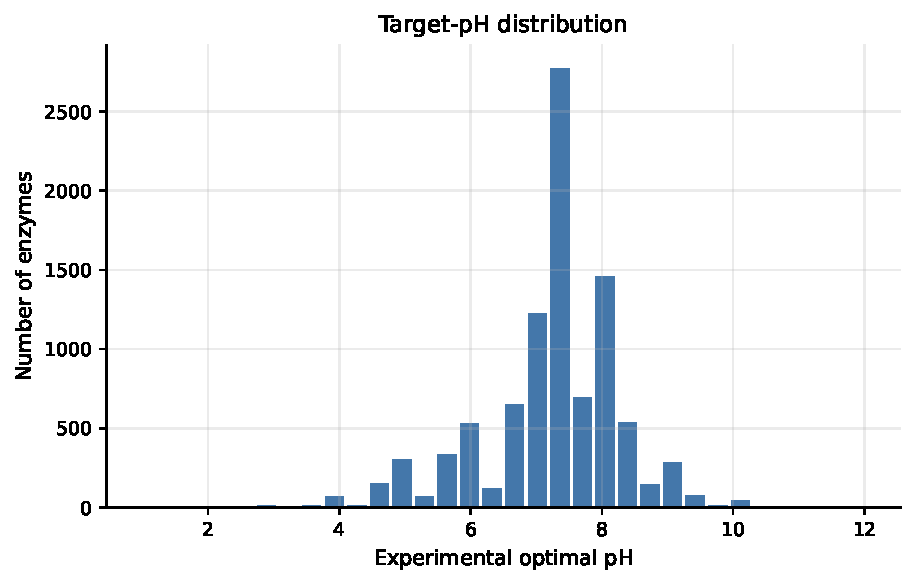
\includegraphics[width=0.78\textwidth]{figures/target_ph_distribution.pdf}
    \caption{Distribution of experimentally measured enzyme optimal-pH values in the cleaned dataset.}
    \label{fig:target-ph-distribution}
\end{figure}

\begin{figure}[htbp]
    \centering
    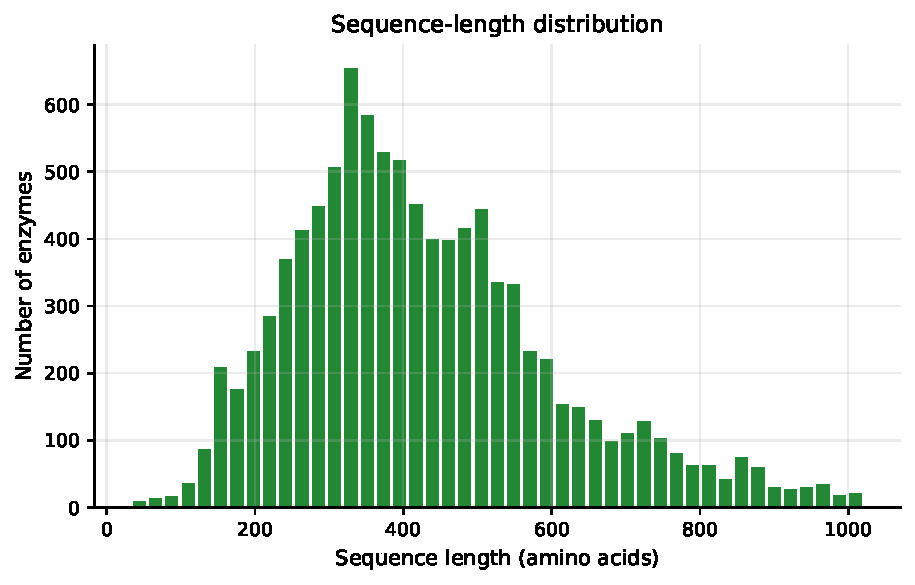
\includegraphics[width=0.78\textwidth]{figures/sequence_length_distribution.pdf}
    \caption{Distribution of amino-acid sequence lengths in the cleaned dataset.}
    \label{fig:sequence-length-distribution}
\end{figure}

\begin{figure}[htbp]
    \centering
    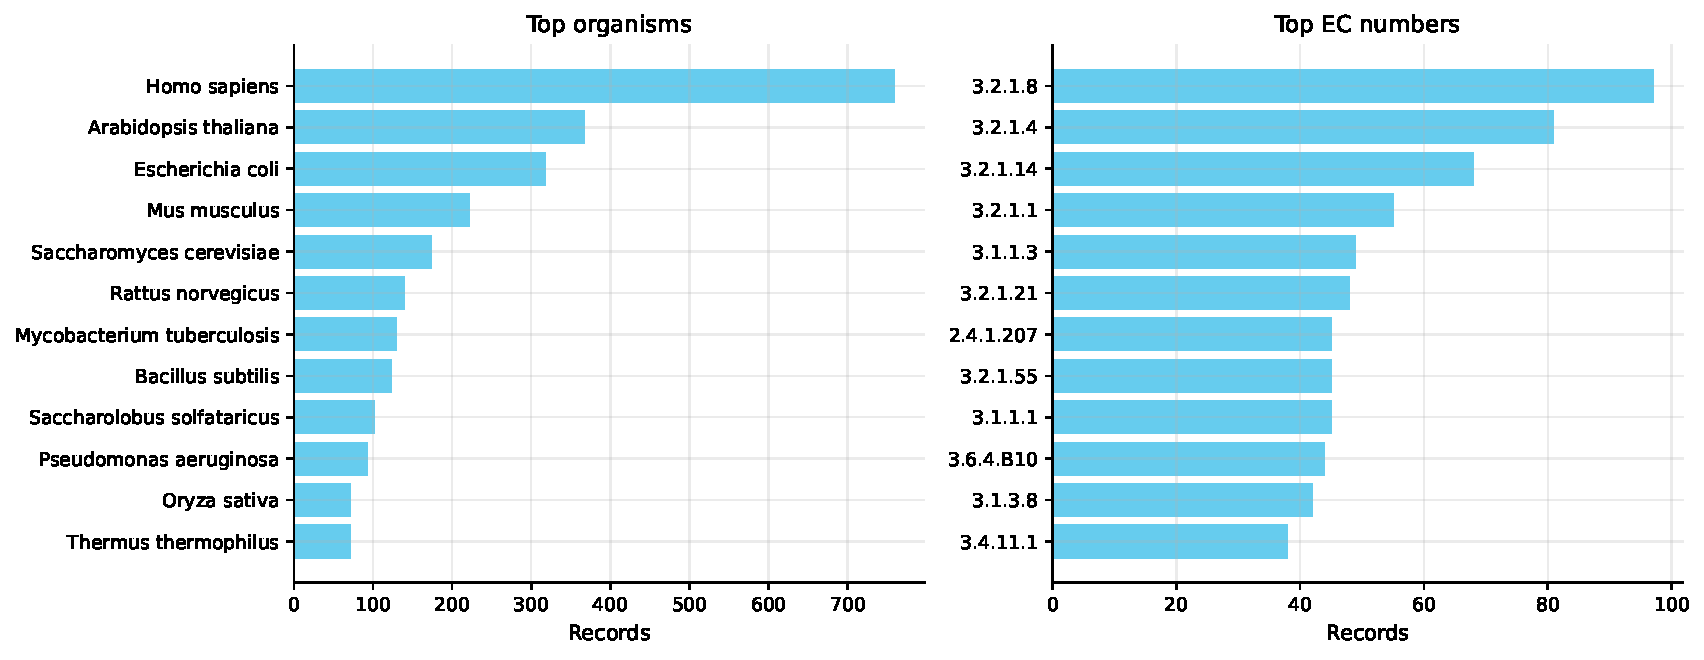
\includegraphics[width=\textwidth]{figures/dataset_composition.pdf}
    \caption{Most frequent organism and EC-number labels in the cleaned dataset.}
    \label{fig:dataset-composition}
\end{figure}


\section{Methodology}
\label{sec:methodology}
Optimal-pH prediction was formulated as a regression task. For an enzyme sequence \(x_i\), each model produced a scalar prediction \(\hat{y}_i\) for the experimentally measured optimal pH \(y_i\). Mean absolute error (MAE) was used as the primary metric because it is directly interpretable in pH units:

\begin{equation}
    \mathrm{MAE} = \frac{1}{n}\sum_{i=1}^{n} |y_i - \hat{y}_i|.
    \label{eq:mae}
\end{equation}

Additional metrics were root mean squared error (RMSE), coefficient of determination (\(R^2\)), Spearman correlation, and Pearson correlation. Bootstrap confidence intervals were estimated on test-set predictions using 500 bootstrap resamples.

Two feature representations were evaluated. The handcrafted representation included sequence length, amino-acid composition over the 20 standard residues, acidic and basic residue fractions, a simple net-charge proxy, hydrophobic, polar, aromatic, and aliphatic residue fractions, GRAVY hydrophobicity, and Biopython-derived physicochemical descriptors where available. The embedding representation used frozen ESM-2 embeddings from \texttt{facebook/esm2\_t6\_8M\_UR50D}. Sequence embeddings were generated by mean-pooling residue-token representations after excluding special and padding tokens. The resulting embedding matrix had shape 9855 by 320.

Generated evaluation strategies included a row-wise random split, an exact-duplicate-safe split, MMseqs2 sequence-cluster-controlled splits at 90\%, 70\%, and 50\% sequence identity, an organism-held-out split, and an EC-held-out split. The row-wise random split assigned records independently to train, validation, and test partitions. The grouped strategies assigned every sequence duplicate, sequence cluster, organism, or EC number to one partition only. MMseqs2 was run with the Windows release available for this analysis using `easy-cluster`, \texttt{--min-seq-id} 0.90, 0.70, or 0.50, \texttt{-c 0.80}, \texttt{--cov-mode 0}, and four threads; the corresponding commands are generated by \texttt{src/clustering.py}. These settings define cluster-disjoint partitions, but cluster membership alone does not prove that every test sequence is below the threshold against every training sequence. A nearest-training-sequence audit using \texttt{scripts/audit\_cluster\_similarity.py} is therefore required before interpreting these splits as homology exclusion. A dataset-provided split was also evaluated for continuity with the input file, but it is not treated as a leakage-controlled split.

The regressors were a mandatory mean predictor, a training-median predictor, ridge regression, random forest regression, and histogram gradient boosting regression. Hyperparameters were fixed before evaluation from \texttt{config/default.yaml}; no model or hyperparameter was selected using test-set performance. The validation partition was retained as a protocol check and for future tuning, but the reported winners are descriptive rankings by test MAE, not validation-selected final models. Training and validation records were not combined before fitting, so every reported test prediction comes from a model fitted on the designated training partition only. All model and split generation used seed 42; the random forest and histogram gradient boosting estimators received this seed, and bootstrap intervals used seed 42. Scalers and imputers were fitted only on the training partition inside scikit-learn pipelines.

Bootstrap intervals resampled individual test rows, so they quantify row-level uncertainty and may be optimistic when related proteins have dependent errors. Paired Wilcoxon comparisons likewise operate at the row level; Holm correction addresses multiplicity but not dependence. These limitations motivate reporting the paired MAE differences directly and treating the inferential results as exploratory.


\section{Experimental Setup}
\label{sec:experiments}
Experiments compared handcrafted sequence features and frozen ESM-2 embeddings across the implemented split strategies. For generated splits, the random split contained 6898 training records, 1478 validation records, and 1479 test records. The exact-duplicate-safe split contained 6895 training, 1480 validation, and 1480 test records. The MMseqs2 90\% cluster-safe split contained 6902 training, 1480 validation, and 1473 test records, with 9025 sequence clusters and no cluster appearing in more than one partition. The organism-held-out split contained 6899 training, 1478 validation, and 1478 test records, with no organism label appearing in more than one partition.

The row-wise random split had 39 exact-duplicate leakage groups, meaning 39 distinct sequence groups crossed partitions. Across the full dataset, 81 distinct sequence groups contained repeated rows, and 41 of those groups had conflicting pHopt labels. Conflicting labels were retained rather than averaged because they may reflect different assay conditions or annotation errors; the exact-duplicate-safe split prevents the same sequence group from crossing partitions, but does not resolve within-group label disagreement.

Ridge regression used \(\alpha = 1.0\). Random forest regression used 300 trees and all available worker processes. Histogram gradient boosting used 300 iterations and learning rate 0.05. ESM-2 embeddings were generated in Google Colab on CUDA with batch size 16 and maximum sequence length 1022 amino acids.

The MMseqs2 50\% and 70\% cluster-safe splits contained 6872/1439/1544 and 6908/1466/1481 training/validation/test records, respectively. The EC-held-out split contained 6899 training, 1478 validation, and 1478 test records, with no EC number appearing in more than one partition. A separate nearest-training-sequence similarity audit is specified in \texttt{scripts/audit\_cluster\_similarity.py}; until it is run with the exact MMseqs2 executable, these are described as cluster-disjoint rather than verified homology-excluded splits. The compact main-results table is included as Table~\ref{tab:model-comparison}. Exhaustive model and split results are provided in the supplementary outputs. Performance by pH range is included as Table~\ref{tab:performance-by-ph-range}; acidic means pH $<6$, near-neutral means $6\leq\mathrm{pH}\leq8$, and alkaline means pH $>8$.

\begin{table}
\caption{Best non-mean model by feature group and split strategy; MAE is shown with a row-level bootstrap 95\% confidence interval.}
\label{tab:model-comparison}
\begin{tabular}{lllrl}
\toprule
Feature group & Split strategy & Model & n examples & MAE (95\% CI) \\
\midrule
ESM-2 embeddings & MMseqs2 50\% & Histogram gradient boosting & 1544 & 0.682 [0.650, 0.717] \\
ESM-2 embeddings & MMseqs2 70\% & Histogram gradient boosting & 1481 & 0.628 [0.598, 0.661] \\
ESM-2 embeddings & MMseqs2 90\% & Histogram gradient boosting & 1473 & 0.615 [0.583, 0.647] \\
ESM-2 embeddings & Dataset-provided & Random forest & 1971 & 0.603 [0.579, 0.630] \\
ESM-2 embeddings & EC-number-held-out & Random forest & 1478 & 0.832 [0.791, 0.877] \\
ESM-2 embeddings & Exact-duplicate-safe & Histogram gradient boosting & 1480 & 0.603 [0.575, 0.642] \\
ESM-2 embeddings & Organism-held-out & Random forest & 1478 & 0.536 [0.508, 0.561] \\
ESM-2 embeddings & Random & Random forest & 1479 & 0.625 [0.593, 0.657] \\
Handcrafted & MMseqs2 50\% & Random forest & 1544 & 0.738 [0.705, 0.776] \\
Handcrafted & MMseqs2 70\% & Random forest & 1481 & 0.695 [0.663, 0.729] \\
Handcrafted & MMseqs2 90\% & Random forest & 1473 & 0.681 [0.647, 0.717] \\
Handcrafted & Dataset-provided & Random forest & 1971 & 0.673 [0.647, 0.701] \\
Handcrafted & EC-number-held-out & Random forest & 1478 & 0.884 [0.849, 0.929] \\
Handcrafted & Exact-duplicate-safe & Random forest & 1480 & 0.664 [0.633, 0.702] \\
Handcrafted & Organism-held-out & Random forest & 1478 & 0.594 [0.564, 0.623] \\
Handcrafted & Random & Random forest & 1479 & 0.698 [0.663, 0.734] \\
\bottomrule
\end{tabular}
\end{table}



\section{Results}
\label{sec:results}
Across all non-mean regressors and split strategies, frozen ESM-2 embeddings achieved lower test MAE than handcrafted sequence features. On the generated random split, the best ESM-2 model was random forest regression with MAE 0.6250 and 95\% bootstrap CI [0.5930, 0.6574]. The corresponding handcrafted random forest model had MAE 0.6984. On the MMseqs2 90\% cluster-safe split, the best ESM-2 model was histogram gradient boosting with MAE 0.6148 and 95\% bootstrap CI [0.5826, 0.6474]. The corresponding handcrafted histogram gradient boosting model had MAE 0.7052.

The current 90\% cluster-safe split did not produce the expected degradation relative to the generated random split. For example, ESM-2 random forest regression had MAE 0.6250 on the generated random split and 0.6164 on the 90\% cluster-safe split. ESM-2 histogram gradient boosting had MAE 0.6335 on the generated random split and 0.6148 on the 90\% cluster-safe split. These results do not support a strong leakage penalty at the 90\% sequence-identity clustering threshold, but they should not be interpreted as evidence that leakage is unimportant. At lower identities, ESM-2 histogram gradient boosting reached MAE 0.6282 at 70\% and 0.6822 at 50\%, showing the expected degradation as the held-out sequences become more distant.

The organism-held-out split also showed lower MAE than the generated random split. ESM-2 random forest regression achieved MAE 0.5360 with 95\% bootstrap CI [0.5079, 0.5609], and ESM-2 histogram gradient boosting achieved MAE 0.5386 with 95\% bootstrap CI [0.5111, 0.5636]. However, the organism-held-out test set had a narrower target distribution than the generated random test set: the target-pH standard deviation was 0.9477 for the organism-held-out test set versus 1.1845 for the generated random test set. This difference likely contributes to the lower MAE and should be considered when interpreting organism generalization.

On the EC-held-out split, ESM-2 random forest achieved the best test MAE at 0.8321 with 95\% bootstrap CI [0.7913, 0.8773]. ESM-2 ridge regression achieved MAE 0.8395 [0.8028, 0.8808], while the best handcrafted model, random forest, achieved MAE 0.8844. The higher EC-held-out errors indicate that generalization across enzyme classes is harder than the current random and sequence-cluster evaluations.

Paired test-set comparisons of absolute error showed lower error for ESM-2 embeddings than handcrafted features for all non-mean regressors across all available split strategies. Wilcoxon test results were written to \texttt{outputs/metrics/paired\_feature\_group\_comparisons.csv}. Holm--Bonferroni adjustment was applied across the full family of 32 paired tests; all 24 non-mean comparisons remained significant at adjusted \(\alpha=0.05\), while mean-predictor comparisons were unchanged because their paired errors are identical.

\begin{figure}[htbp]
    \centering
    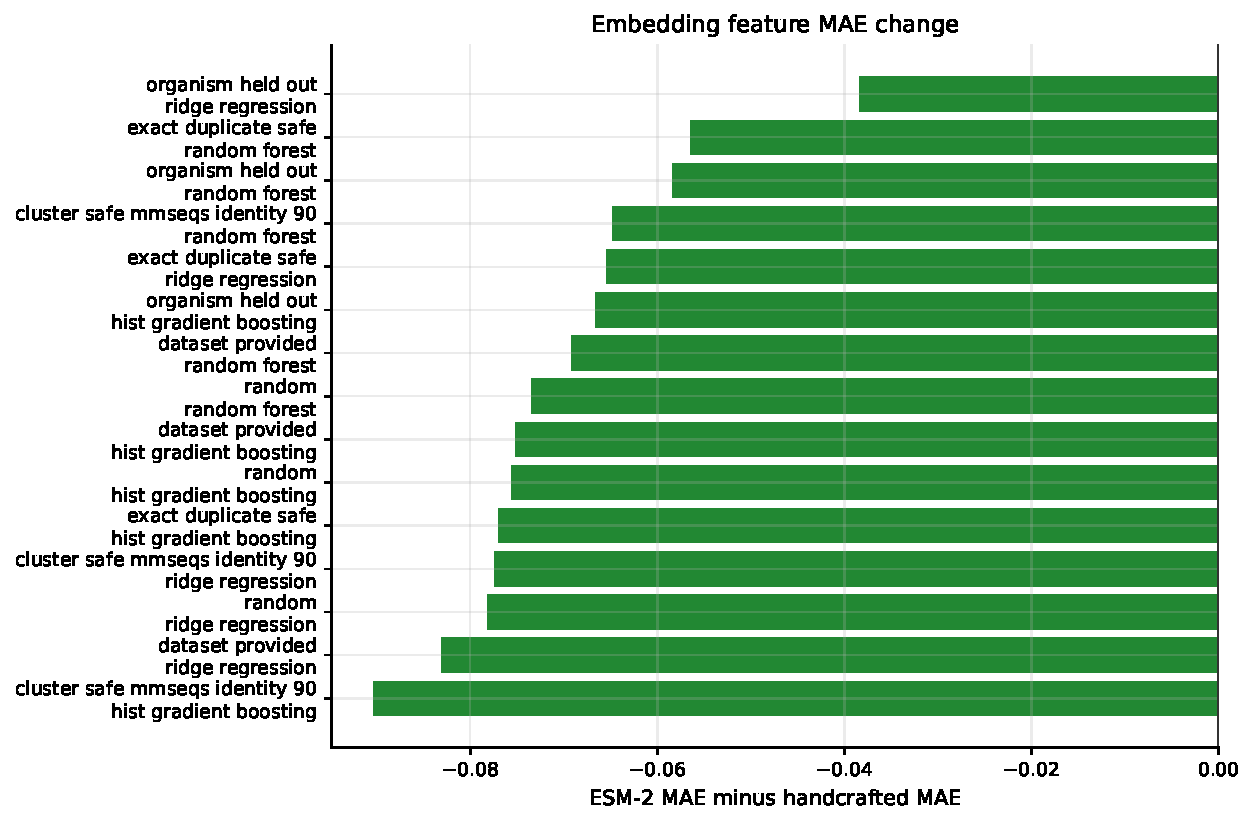
\includegraphics[width=\textwidth]{figures/embedding_vs_handcrafted_mae_change.pdf}
    \caption{Change in test MAE when replacing handcrafted sequence features with frozen ESM-2 embeddings. Negative values indicate lower MAE for embeddings.}
    \label{fig:embedding-vs-handcrafted}
\end{figure}

\begin{figure}[htbp]
    \centering
    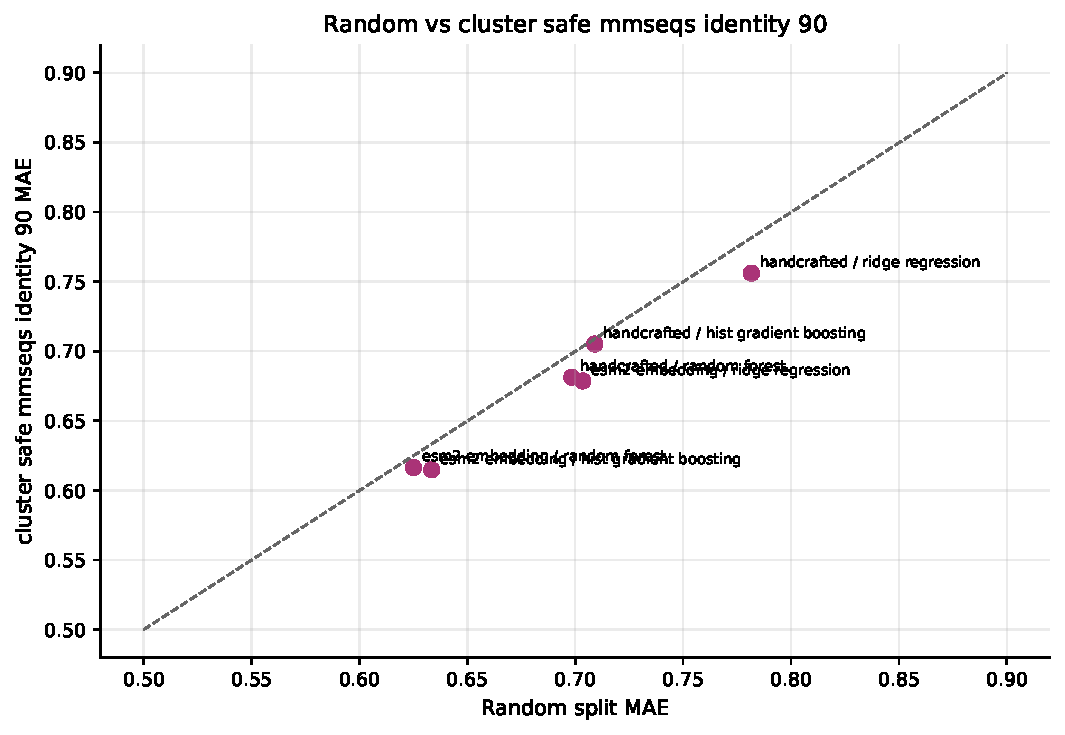
\includegraphics[width=0.78\textwidth]{figures/random_vs_cluster_mae.pdf}
    \caption{Selected comparison of generated random-split MAE and MMseqs2 90\% cluster-safe split MAE for evaluated models. The 70\% and 50\% cluster-safe results are reported in the text and model-comparison tables but are not plotted here. The dashed line indicates equal MAE under both split strategies.}
    \label{fig:random-vs-cluster}
\end{figure}

\begin{figure}[htbp]
    \centering
    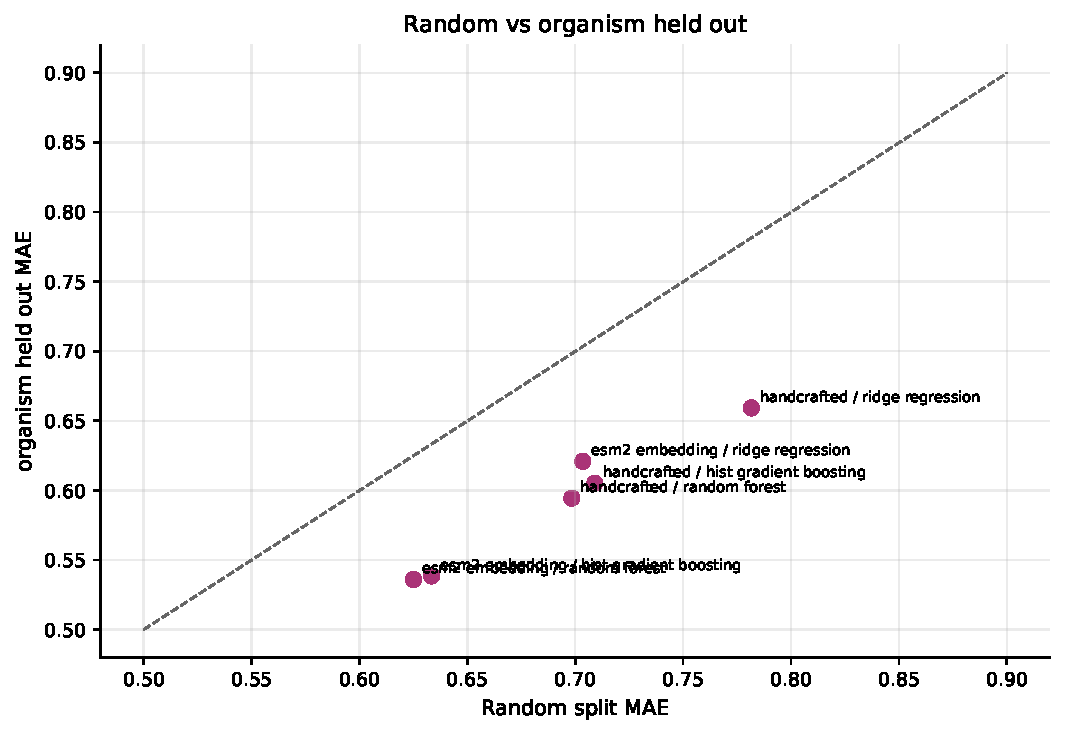
\includegraphics[width=0.78\textwidth]{figures/random_vs_organism_mae.pdf}
    \caption{Selected comparison of generated random-split MAE and organism-held-out split MAE for evaluated models. The cluster-identity and EC-held-out comparisons are reported separately in the text and tables. The organism-held-out test set has a narrower target-pH distribution than the generated random test set.}
    \label{fig:random-vs-organism}
\end{figure}

\begin{figure}[htbp]
    \centering
    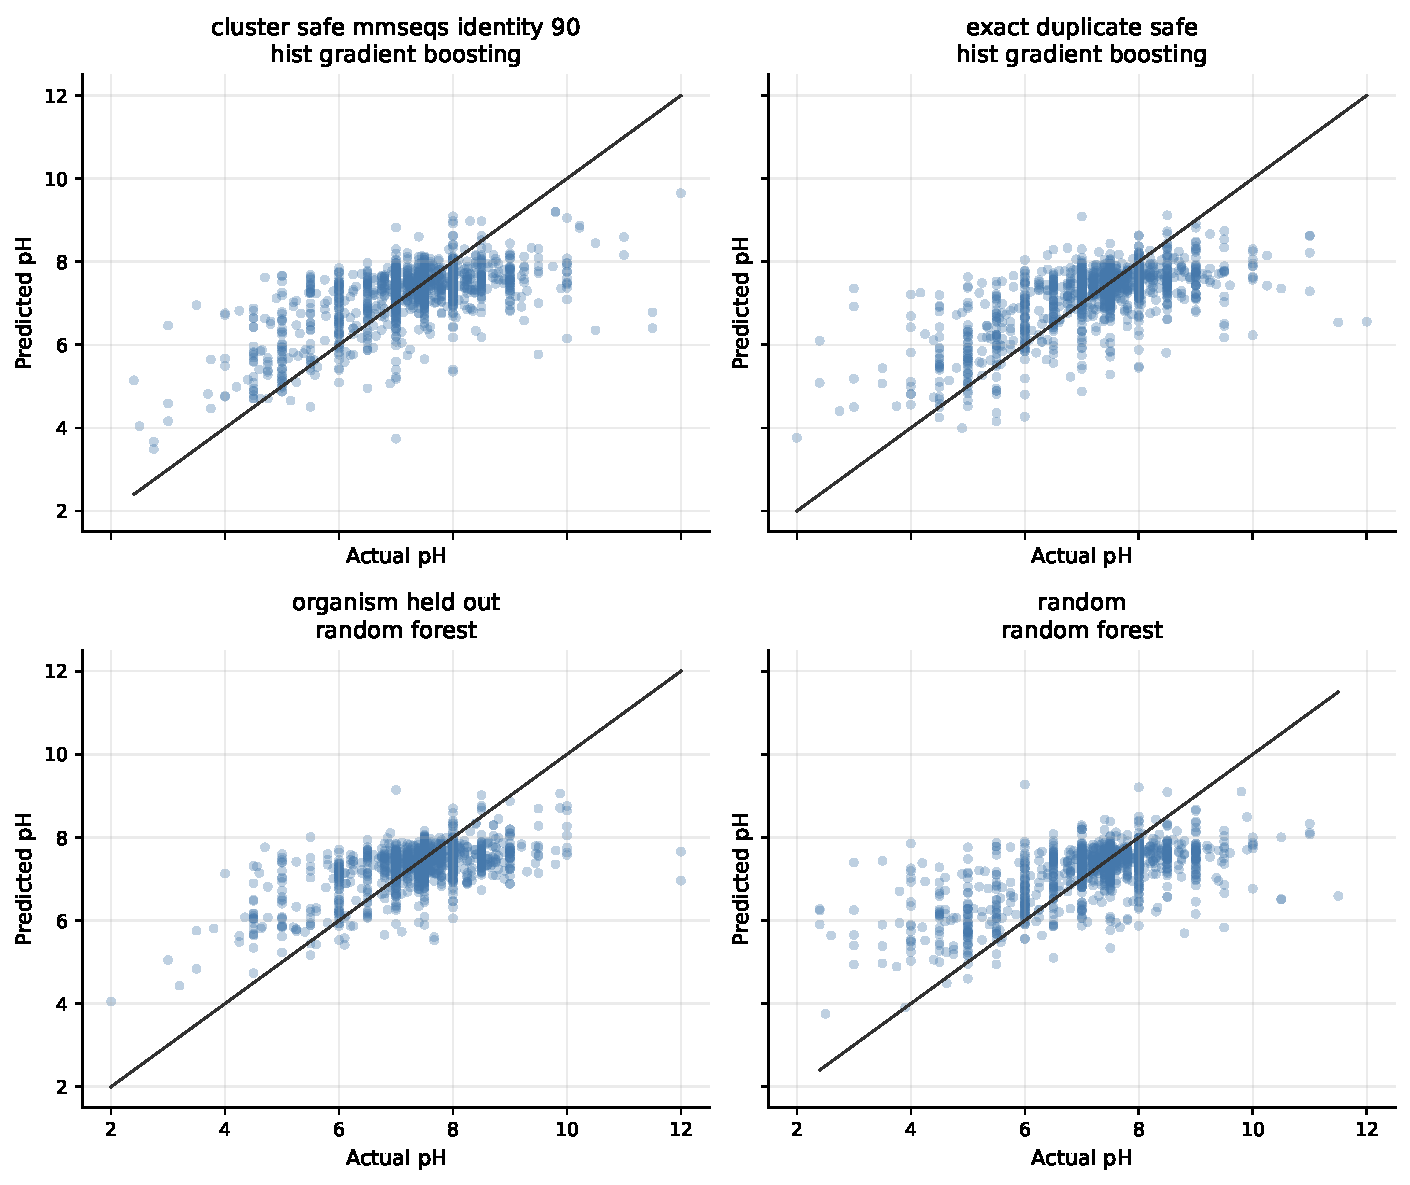
\includegraphics[width=\textwidth]{figures/actual_vs_predicted_best_embedding_models.pdf}
    \caption{Actual versus predicted optimal pH for the selected best ESM-2 embedding models represented in the generated prediction diagnostics. The full set of split-specific metrics, including 50\%, 70\%, and EC-held-out evaluations, is reported in the tables.}
    \label{fig:actual-vs-predicted}
\end{figure}

\begin{longtable}{llllrrrr}
\caption{Test-set performance stratified by experimental optimal-pH range.} \label{tab:performance-by-ph-range} \\
\toprule
feature\_group & split\_strategy & model & ph\_range & n\_examples & mae & rmse & bias \\
\midrule
\endfirsthead
\caption[]{Test-set performance stratified by experimental optimal-pH range.} \\
\toprule
feature\_group & split\_strategy & model & ph\_range & n\_examples & mae & rmse & bias \\
\midrule
\endhead
\midrule
\multicolumn{8}{r}{Continued on next page} \\
\midrule
\endfoot
\bottomrule
\endlastfoot
esm2\_embedding & cluster\_safe\_mmseqs\_identity\_50 & hist\_gradient\_boosting & acidic & 203 & 1.592800 & 1.850100 & 1.578400 \\
esm2\_embedding & cluster\_safe\_mmseqs\_identity\_50 & hist\_gradient\_boosting & alkaline & 174 & 1.303800 & 1.602200 & -1.300900 \\
esm2\_embedding & cluster\_safe\_mmseqs\_identity\_50 & hist\_gradient\_boosting & near\_neutral & 1167 & 0.431100 & 0.582900 & 0.019400 \\
esm2\_embedding & cluster\_safe\_mmseqs\_identity\_50 & mean\_predictor & acidic & 203 & 2.436900 & 2.580400 & 2.436900 \\
esm2\_embedding & cluster\_safe\_mmseqs\_identity\_50 & mean\_predictor & alkaline & 174 & 1.569500 & 1.716700 & -1.569500 \\
esm2\_embedding & cluster\_safe\_mmseqs\_identity\_50 & mean\_predictor & near\_neutral & 1167 & 0.468000 & 0.578800 & -0.027400 \\
esm2\_embedding & cluster\_safe\_mmseqs\_identity\_50 & median\_predictor & acidic & 203 & 2.669300 & 2.800900 & 2.669300 \\
esm2\_embedding & cluster\_safe\_mmseqs\_identity\_50 & median\_predictor & alkaline & 174 & 1.337100 & 1.507100 & -1.337100 \\
esm2\_embedding & cluster\_safe\_mmseqs\_identity\_50 & median\_predictor & near\_neutral & 1167 & 0.426300 & 0.613400 & 0.205000 \\
esm2\_embedding & cluster\_safe\_mmseqs\_identity\_50 & random\_forest & acidic & 203 & 1.655300 & 1.891000 & 1.649100 \\
esm2\_embedding & cluster\_safe\_mmseqs\_identity\_50 & random\_forest & alkaline & 174 & 1.340800 & 1.630600 & -1.340800 \\
esm2\_embedding & cluster\_safe\_mmseqs\_identity\_50 & random\_forest & near\_neutral & 1167 & 0.419300 & 0.568200 & 0.003800 \\
esm2\_embedding & cluster\_safe\_mmseqs\_identity\_50 & ridge\_regression & acidic & 203 & 1.561300 & 1.821200 & 1.545100 \\
esm2\_embedding & cluster\_safe\_mmseqs\_identity\_50 & ridge\_regression & alkaline & 174 & 1.318700 & 1.610900 & -1.316300 \\
esm2\_embedding & cluster\_safe\_mmseqs\_identity\_50 & ridge\_regression & near\_neutral & 1167 & 0.491100 & 0.647300 & -0.002300 \\
esm2\_embedding & cluster\_safe\_mmseqs\_identity\_70 & hist\_gradient\_boosting & acidic & 149 & 1.146300 & 1.453900 & 1.069800 \\
esm2\_embedding & cluster\_safe\_mmseqs\_identity\_70 & hist\_gradient\_boosting & alkaline & 214 & 1.306100 & 1.495500 & -1.301000 \\
esm2\_embedding & cluster\_safe\_mmseqs\_identity\_70 & hist\_gradient\_boosting & near\_neutral & 1118 & 0.429400 & 0.569900 & 0.062600 \\
esm2\_embedding & cluster\_safe\_mmseqs\_identity\_70 & mean\_predictor & acidic & 149 & 2.427800 & 2.559900 & 2.427800 \\
esm2\_embedding & cluster\_safe\_mmseqs\_identity\_70 & mean\_predictor & alkaline & 214 & 1.626200 & 1.736500 & -1.626200 \\
esm2\_embedding & cluster\_safe\_mmseqs\_identity\_70 & mean\_predictor & near\_neutral & 1118 & 0.441800 & 0.543200 & -0.049600 \\
esm2\_embedding & cluster\_safe\_mmseqs\_identity\_70 & median\_predictor & acidic & 149 & 2.696900 & 2.816500 & 2.696900 \\
esm2\_embedding & cluster\_safe\_mmseqs\_identity\_70 & median\_predictor & alkaline & 214 & 1.357000 & 1.487400 & -1.357000 \\
esm2\_embedding & cluster\_safe\_mmseqs\_identity\_70 & median\_predictor & near\_neutral & 1118 & 0.416500 & 0.583800 & 0.219500 \\
esm2\_embedding & cluster\_safe\_mmseqs\_identity\_70 & random\_forest & acidic & 149 & 1.223200 & 1.528000 & 1.199100 \\
esm2\_embedding & cluster\_safe\_mmseqs\_identity\_70 & random\_forest & alkaline & 214 & 1.354100 & 1.530600 & -1.352700 \\
esm2\_embedding & cluster\_safe\_mmseqs\_identity\_70 & random\_forest & near\_neutral & 1118 & 0.412100 & 0.546400 & 0.050200 \\
esm2\_embedding & cluster\_safe\_mmseqs\_identity\_70 & ridge\_regression & acidic & 149 & 1.208000 & 1.478700 & 1.157100 \\
esm2\_embedding & cluster\_safe\_mmseqs\_identity\_70 & ridge\_regression & alkaline & 214 & 1.345300 & 1.538600 & -1.329800 \\
esm2\_embedding & cluster\_safe\_mmseqs\_identity\_70 & ridge\_regression & near\_neutral & 1118 & 0.485800 & 0.619800 & 0.059700 \\
esm2\_embedding & cluster\_safe\_mmseqs\_identity\_90 & hist\_gradient\_boosting & acidic & 152 & 1.170000 & 1.407100 & 1.135700 \\
esm2\_embedding & cluster\_safe\_mmseqs\_identity\_90 & hist\_gradient\_boosting & alkaline & 220 & 1.222100 & 1.441100 & -1.209400 \\
esm2\_embedding & cluster\_safe\_mmseqs\_identity\_90 & hist\_gradient\_boosting & near\_neutral & 1101 & 0.416900 & 0.566000 & 0.044400 \\
esm2\_embedding & cluster\_safe\_mmseqs\_identity\_90 & mean\_predictor & acidic & 152 & 2.326100 & 2.422300 & 2.326100 \\
esm2\_embedding & cluster\_safe\_mmseqs\_identity\_90 & mean\_predictor & alkaline & 220 & 1.624700 & 1.756700 & -1.624700 \\
esm2\_embedding & cluster\_safe\_mmseqs\_identity\_90 & mean\_predictor & near\_neutral & 1101 & 0.448400 & 0.548600 & -0.079200 \\
esm2\_embedding & cluster\_safe\_mmseqs\_identity\_90 & median\_predictor & acidic & 152 & 2.607000 & 2.693200 & 2.607000 \\
esm2\_embedding & cluster\_safe\_mmseqs\_identity\_90 & median\_predictor & alkaline & 220 & 1.343700 & 1.500700 & -1.343700 \\
esm2\_embedding & cluster\_safe\_mmseqs\_identity\_90 & median\_predictor & near\_neutral & 1101 & 0.417600 & 0.579100 & 0.201700 \\
esm2\_embedding & cluster\_safe\_mmseqs\_identity\_90 & random\_forest & acidic & 152 & 1.257900 & 1.483000 & 1.248500 \\
esm2\_embedding & cluster\_safe\_mmseqs\_identity\_90 & random\_forest & alkaline & 220 & 1.276900 & 1.487900 & -1.271700 \\
esm2\_embedding & cluster\_safe\_mmseqs\_identity\_90 & random\_forest & near\_neutral & 1101 & 0.395900 & 0.542700 & 0.033900 \\
esm2\_embedding & cluster\_safe\_mmseqs\_identity\_90 & ridge\_regression & acidic & 152 & 1.239100 & 1.463100 & 1.199300 \\
esm2\_embedding & cluster\_safe\_mmseqs\_identity\_90 & ridge\_regression & alkaline & 220 & 1.307300 & 1.531200 & -1.295500 \\
esm2\_embedding & cluster\_safe\_mmseqs\_identity\_90 & ridge\_regression & near\_neutral & 1101 & 0.475600 & 0.616600 & 0.046100 \\
esm2\_embedding & dataset\_provided & hist\_gradient\_boosting & acidic & 218 & 1.134400 & 1.400400 & 1.055500 \\
esm2\_embedding & dataset\_provided & hist\_gradient\_boosting & alkaline & 285 & 1.178900 & 1.373900 & -1.174000 \\
esm2\_embedding & dataset\_provided & hist\_gradient\_boosting & near\_neutral & 1468 & 0.425900 & 0.573400 & 0.023600 \\
esm2\_embedding & dataset\_provided & mean\_predictor & acidic & 218 & 2.288700 & 2.405900 & 2.288700 \\
esm2\_embedding & dataset\_provided & mean\_predictor & alkaline & 285 & 1.636900 & 1.744600 & -1.636900 \\
esm2\_embedding & dataset\_provided & mean\_predictor & near\_neutral & 1468 & 0.481100 & 0.584000 & -0.072400 \\
esm2\_embedding & dataset\_provided & median\_predictor & acidic & 218 & 2.578000 & 2.682700 & 2.578000 \\
esm2\_embedding & dataset\_provided & median\_predictor & alkaline & 285 & 1.347500 & 1.476500 & -1.347500 \\
esm2\_embedding & dataset\_provided & median\_predictor & near\_neutral & 1468 & 0.442700 & 0.618800 & 0.216900 \\
esm2\_embedding & dataset\_provided & random\_forest & acidic & 218 & 1.172800 & 1.405800 & 1.144900 \\
esm2\_embedding & dataset\_provided & random\_forest & alkaline & 285 & 1.213600 & 1.396400 & -1.213200 \\
esm2\_embedding & dataset\_provided & random\_forest & near\_neutral & 1468 & 0.400500 & 0.544000 & 0.014400 \\
esm2\_embedding & dataset\_provided & ridge\_regression & acidic & 218 & 1.220600 & 1.473000 & 1.153800 \\
esm2\_embedding & dataset\_provided & ridge\_regression & alkaline & 285 & 1.246200 & 1.427300 & -1.234000 \\
esm2\_embedding & dataset\_provided & ridge\_regression & near\_neutral & 1468 & 0.482000 & 0.632600 & 0.011900 \\
esm2\_embedding & ec\_held\_out & hist\_gradient\_boosting & acidic & 360 & 1.351100 & 1.624400 & 1.312000 \\
esm2\_embedding & ec\_held\_out & hist\_gradient\_boosting & alkaline & 138 & 1.875700 & 2.258500 & -1.875700 \\
esm2\_embedding & ec\_held\_out & hist\_gradient\_boosting & near\_neutral & 980 & 0.507700 & 0.683100 & -0.030100 \\
esm2\_embedding & ec\_held\_out & mean\_predictor & acidic & 360 & 2.449400 & 2.544600 & 2.449400 \\
esm2\_embedding & ec\_held\_out & mean\_predictor & alkaline & 138 & 1.677500 & 1.859800 & -1.677500 \\
esm2\_embedding & ec\_held\_out & mean\_predictor & near\_neutral & 980 & 0.522600 & 0.683400 & 0.249400 \\
esm2\_embedding & ec\_held\_out & median\_predictor & acidic & 360 & 2.595800 & 2.685800 & 2.595800 \\
esm2\_embedding & ec\_held\_out & median\_predictor & alkaline & 138 & 1.531100 & 1.728900 & -1.531100 \\
esm2\_embedding & ec\_held\_out & median\_predictor & near\_neutral & 980 & 0.541600 & 0.749400 & 0.395800 \\
esm2\_embedding & ec\_held\_out & random\_forest & acidic & 360 & 1.371000 & 1.620700 & 1.353100 \\
esm2\_embedding & ec\_held\_out & random\_forest & alkaline & 138 & 1.918300 & 2.297400 & -1.918300 \\
esm2\_embedding & ec\_held\_out & random\_forest & near\_neutral & 980 & 0.481200 & 0.650700 & -0.023900 \\
esm2\_embedding & ec\_held\_out & ridge\_regression & acidic & 360 & 1.317800 & 1.556200 & 1.267400 \\
esm2\_embedding & ec\_held\_out & ridge\_regression & alkaline & 138 & 1.881300 & 2.218200 & -1.881200 \\
esm2\_embedding & ec\_held\_out & ridge\_regression & near\_neutral & 980 & 0.517100 & 0.672300 & -0.054500 \\
esm2\_embedding & exact\_duplicate\_safe & hist\_gradient\_boosting & acidic & 174 & 1.091700 & 1.348400 & 1.005200 \\
esm2\_embedding & exact\_duplicate\_safe & hist\_gradient\_boosting & alkaline & 217 & 1.189500 & 1.431300 & -1.179500 \\
esm2\_embedding & exact\_duplicate\_safe & hist\_gradient\_boosting & near\_neutral & 1089 & 0.407800 & 0.558800 & 0.027800 \\
esm2\_embedding & exact\_duplicate\_safe & mean\_predictor & acidic & 174 & 2.268400 & 2.378400 & 2.268400 \\
esm2\_embedding & exact\_duplicate\_safe & mean\_predictor & alkaline & 217 & 1.606000 & 1.732900 & -1.606000 \\
esm2\_embedding & exact\_duplicate\_safe & mean\_predictor & near\_neutral & 1089 & 0.455300 & 0.552400 & -0.084300 \\
esm2\_embedding & exact\_duplicate\_safe & median\_predictor & acidic & 174 & 2.546800 & 2.645200 & 2.546800 \\
esm2\_embedding & exact\_duplicate\_safe & median\_predictor & alkaline & 217 & 1.327600 & 1.478600 & -1.327600 \\
esm2\_embedding & exact\_duplicate\_safe & median\_predictor & near\_neutral & 1089 & 0.413600 & 0.579400 & 0.194100 \\
esm2\_embedding & exact\_duplicate\_safe & random\_forest & acidic & 174 & 1.173300 & 1.410800 & 1.143400 \\
esm2\_embedding & exact\_duplicate\_safe & random\_forest & alkaline & 217 & 1.231900 & 1.476300 & -1.225600 \\
esm2\_embedding & exact\_duplicate\_safe & random\_forest & near\_neutral & 1089 & 0.392400 & 0.529500 & 0.010100 \\
esm2\_embedding & exact\_duplicate\_safe & ridge\_regression & acidic & 174 & 1.250600 & 1.489300 & 1.160800 \\
esm2\_embedding & exact\_duplicate\_safe & ridge\_regression & alkaline & 217 & 1.283600 & 1.538300 & -1.269000 \\
esm2\_embedding & exact\_duplicate\_safe & ridge\_regression & near\_neutral & 1089 & 0.477100 & 0.619800 & -0.003600 \\
esm2\_embedding & organism\_held\_out & hist\_gradient\_boosting & acidic & 88 & 1.334900 & 1.538400 & 1.312700 \\
esm2\_embedding & organism\_held\_out & hist\_gradient\_boosting & alkaline & 209 & 1.069200 & 1.230100 & -1.046900 \\
esm2\_embedding & organism\_held\_out & hist\_gradient\_boosting & near\_neutral & 1181 & 0.385300 & 0.517200 & 0.049000 \\
esm2\_embedding & organism\_held\_out & mean\_predictor & acidic & 88 & 2.274800 & 2.369300 & 2.274800 \\
esm2\_embedding & organism\_held\_out & mean\_predictor & alkaline & 209 & 1.564500 & 1.656800 & -1.564500 \\
esm2\_embedding & organism\_held\_out & mean\_predictor & near\_neutral & 1181 & 0.442100 & 0.532000 & -0.175400 \\
esm2\_embedding & organism\_held\_out & median\_predictor & acidic & 88 & 2.509000 & 2.595000 & 2.509000 \\
esm2\_embedding & organism\_held\_out & median\_predictor & alkaline & 209 & 1.330300 & 1.437800 & -1.330300 \\
esm2\_embedding & organism\_held\_out & median\_predictor & near\_neutral & 1181 & 0.366800 & 0.505600 & 0.058700 \\
esm2\_embedding & organism\_held\_out & random\_forest & acidic & 88 & 1.418900 & 1.596600 & 1.405900 \\
esm2\_embedding & organism\_held\_out & random\_forest & alkaline & 209 & 1.122900 & 1.270000 & -1.111900 \\
esm2\_embedding & organism\_held\_out & random\_forest & near\_neutral & 1181 & 0.366400 & 0.494500 & 0.020100 \\
esm2\_embedding & organism\_held\_out & ridge\_regression & acidic & 88 & 1.408800 & 1.575100 & 1.394900 \\
esm2\_embedding & organism\_held\_out & ridge\_regression & alkaline & 209 & 1.101100 & 1.317600 & -1.069500 \\
esm2\_embedding & organism\_held\_out & ridge\_regression & near\_neutral & 1181 & 0.477200 & 0.617300 & 0.056400 \\
esm2\_embedding & random & hist\_gradient\_boosting & acidic & 177 & 1.280800 & 1.577900 & 1.248800 \\
esm2\_embedding & random & hist\_gradient\_boosting & alkaline & 200 & 1.240100 & 1.448100 & -1.230700 \\
esm2\_embedding & random & hist\_gradient\_boosting & near\_neutral & 1102 & 0.419400 & 0.570800 & 0.044900 \\
esm2\_embedding & random & mean\_predictor & acidic & 177 & 2.442200 & 2.556400 & 2.442200 \\
esm2\_embedding & random & mean\_predictor & alkaline & 200 & 1.592800 & 1.702700 & -1.592800 \\
esm2\_embedding & random & mean\_predictor & near\_neutral & 1102 & 0.452000 & 0.553600 & -0.079100 \\
esm2\_embedding & random & median\_predictor & acidic & 177 & 2.711200 & 2.814500 & 2.711200 \\
esm2\_embedding & random & median\_predictor & alkaline & 200 & 1.323800 & 1.454200 & -1.323800 \\
esm2\_embedding & random & median\_predictor & near\_neutral & 1102 & 0.415000 & 0.579900 & 0.189900 \\
esm2\_embedding & random & random\_forest & acidic & 177 & 1.363300 & 1.638500 & 1.345700 \\
esm2\_embedding & random & random\_forest & alkaline & 200 & 1.266000 & 1.475800 & -1.258700 \\
esm2\_embedding & random & random\_forest & near\_neutral & 1102 & 0.390100 & 0.536900 & 0.016300 \\
esm2\_embedding & random & ridge\_regression & acidic & 177 & 1.459900 & 1.740700 & 1.414200 \\
esm2\_embedding & random & ridge\_regression & alkaline & 200 & 1.297600 & 1.503000 & -1.286100 \\
esm2\_embedding & random & ridge\_regression & near\_neutral & 1102 & 0.474200 & 0.615900 & 0.028500 \\
handcrafted & cluster\_safe\_mmseqs\_identity\_50 & hist\_gradient\_boosting & acidic & 203 & 1.770000 & 2.032000 & 1.743000 \\
handcrafted & cluster\_safe\_mmseqs\_identity\_50 & hist\_gradient\_boosting & alkaline & 174 & 1.398600 & 1.664500 & -1.398600 \\
handcrafted & cluster\_safe\_mmseqs\_identity\_50 & hist\_gradient\_boosting & near\_neutral & 1167 & 0.464100 & 0.612600 & 0.022300 \\
handcrafted & cluster\_safe\_mmseqs\_identity\_50 & mean\_predictor & acidic & 203 & 2.436900 & 2.580400 & 2.436900 \\
handcrafted & cluster\_safe\_mmseqs\_identity\_50 & mean\_predictor & alkaline & 174 & 1.569500 & 1.716700 & -1.569500 \\
handcrafted & cluster\_safe\_mmseqs\_identity\_50 & mean\_predictor & near\_neutral & 1167 & 0.468000 & 0.578800 & -0.027400 \\
handcrafted & cluster\_safe\_mmseqs\_identity\_50 & median\_predictor & acidic & 203 & 2.669300 & 2.800900 & 2.669300 \\
handcrafted & cluster\_safe\_mmseqs\_identity\_50 & median\_predictor & alkaline & 174 & 1.337100 & 1.507100 & -1.337100 \\
handcrafted & cluster\_safe\_mmseqs\_identity\_50 & median\_predictor & near\_neutral & 1167 & 0.426300 & 0.613400 & 0.205000 \\
handcrafted & cluster\_safe\_mmseqs\_identity\_50 & random\_forest & acidic & 203 & 1.811000 & 2.057100 & 1.793900 \\
handcrafted & cluster\_safe\_mmseqs\_identity\_50 & random\_forest & alkaline & 174 & 1.415900 & 1.668000 & -1.415900 \\
handcrafted & cluster\_safe\_mmseqs\_identity\_50 & random\_forest & near\_neutral & 1167 & 0.449700 & 0.588700 & 0.013700 \\
handcrafted & cluster\_safe\_mmseqs\_identity\_50 & ridge\_regression & acidic & 203 & 1.968400 & 2.185500 & 1.968400 \\
handcrafted & cluster\_safe\_mmseqs\_identity\_50 & ridge\_regression & alkaline & 174 & 1.462400 & 1.699400 & -1.455300 \\
handcrafted & cluster\_safe\_mmseqs\_identity\_50 & ridge\_regression & near\_neutral & 1167 & 0.463400 & 0.599700 & -0.001500 \\
handcrafted & cluster\_safe\_mmseqs\_identity\_70 & hist\_gradient\_boosting & acidic & 149 & 1.540300 & 1.794400 & 1.505600 \\
handcrafted & cluster\_safe\_mmseqs\_identity\_70 & hist\_gradient\_boosting & alkaline & 214 & 1.442800 & 1.612100 & -1.442800 \\
handcrafted & cluster\_safe\_mmseqs\_identity\_70 & hist\_gradient\_boosting & near\_neutral & 1118 & 0.447700 & 0.586000 & 0.035800 \\
handcrafted & cluster\_safe\_mmseqs\_identity\_70 & mean\_predictor & acidic & 149 & 2.427800 & 2.559900 & 2.427800 \\
handcrafted & cluster\_safe\_mmseqs\_identity\_70 & mean\_predictor & alkaline & 214 & 1.626200 & 1.736500 & -1.626200 \\
handcrafted & cluster\_safe\_mmseqs\_identity\_70 & mean\_predictor & near\_neutral & 1118 & 0.441800 & 0.543200 & -0.049600 \\
handcrafted & cluster\_safe\_mmseqs\_identity\_70 & median\_predictor & acidic & 149 & 2.696900 & 2.816500 & 2.696900 \\
handcrafted & cluster\_safe\_mmseqs\_identity\_70 & median\_predictor & alkaline & 214 & 1.357000 & 1.487400 & -1.357000 \\
handcrafted & cluster\_safe\_mmseqs\_identity\_70 & median\_predictor & near\_neutral & 1118 & 0.416500 & 0.583800 & 0.219500 \\
handcrafted & cluster\_safe\_mmseqs\_identity\_70 & random\_forest & acidic & 149 & 1.555300 & 1.819600 & 1.530600 \\
handcrafted & cluster\_safe\_mmseqs\_identity\_70 & random\_forest & alkaline & 214 & 1.477100 & 1.653900 & -1.477100 \\
handcrafted & cluster\_safe\_mmseqs\_identity\_70 & random\_forest & near\_neutral & 1118 & 0.431100 & 0.565600 & 0.020400 \\
handcrafted & cluster\_safe\_mmseqs\_identity\_70 & ridge\_regression & acidic & 149 & 1.832900 & 2.031800 & 1.832900 \\
handcrafted & cluster\_safe\_mmseqs\_identity\_70 & ridge\_regression & alkaline & 214 & 1.545700 & 1.713400 & -1.542800 \\
handcrafted & cluster\_safe\_mmseqs\_identity\_70 & ridge\_regression & near\_neutral & 1118 & 0.453300 & 0.573100 & -0.021800 \\
handcrafted & cluster\_safe\_mmseqs\_identity\_90 & hist\_gradient\_boosting & acidic & 152 & 1.445900 & 1.652200 & 1.408100 \\
handcrafted & cluster\_safe\_mmseqs\_identity\_90 & hist\_gradient\_boosting & alkaline & 220 & 1.391300 & 1.603600 & -1.389600 \\
handcrafted & cluster\_safe\_mmseqs\_identity\_90 & hist\_gradient\_boosting & near\_neutral & 1101 & 0.465800 & 0.620800 & 0.043500 \\
handcrafted & cluster\_safe\_mmseqs\_identity\_90 & mean\_predictor & acidic & 152 & 2.326100 & 2.422300 & 2.326100 \\
handcrafted & cluster\_safe\_mmseqs\_identity\_90 & mean\_predictor & alkaline & 220 & 1.624700 & 1.756700 & -1.624700 \\
handcrafted & cluster\_safe\_mmseqs\_identity\_90 & mean\_predictor & near\_neutral & 1101 & 0.448400 & 0.548600 & -0.079200 \\
handcrafted & cluster\_safe\_mmseqs\_identity\_90 & median\_predictor & acidic & 152 & 2.607000 & 2.693200 & 2.607000 \\
handcrafted & cluster\_safe\_mmseqs\_identity\_90 & median\_predictor & alkaline & 220 & 1.343700 & 1.500700 & -1.343700 \\
handcrafted & cluster\_safe\_mmseqs\_identity\_90 & median\_predictor & near\_neutral & 1101 & 0.417600 & 0.579100 & 0.201700 \\
handcrafted & cluster\_safe\_mmseqs\_identity\_90 & random\_forest & acidic & 152 & 1.477800 & 1.674400 & 1.464900 \\
handcrafted & cluster\_safe\_mmseqs\_identity\_90 & random\_forest & alkaline & 220 & 1.387400 & 1.601300 & -1.385000 \\
handcrafted & cluster\_safe\_mmseqs\_identity\_90 & random\_forest & near\_neutral & 1101 & 0.430200 & 0.576900 & 0.020400 \\
handcrafted & cluster\_safe\_mmseqs\_identity\_90 & ridge\_regression & acidic & 152 & 1.769100 & 1.890400 & 1.769100 \\
handcrafted & cluster\_safe\_mmseqs\_identity\_90 & ridge\_regression & alkaline & 220 & 1.480000 & 1.698000 & -1.472100 \\
handcrafted & cluster\_safe\_mmseqs\_identity\_90 & ridge\_regression & near\_neutral & 1101 & 0.471500 & 0.603200 & 0.002000 \\
handcrafted & dataset\_provided & hist\_gradient\_boosting & acidic & 218 & 1.392800 & 1.625900 & 1.345100 \\
handcrafted & dataset\_provided & hist\_gradient\_boosting & alkaline & 285 & 1.346700 & 1.516900 & -1.346100 \\
handcrafted & dataset\_provided & hist\_gradient\_boosting & near\_neutral & 1468 & 0.455800 & 0.598800 & 0.008700 \\
handcrafted & dataset\_provided & mean\_predictor & acidic & 218 & 2.288700 & 2.405900 & 2.288700 \\
handcrafted & dataset\_provided & mean\_predictor & alkaline & 285 & 1.636900 & 1.744600 & -1.636900 \\
handcrafted & dataset\_provided & mean\_predictor & near\_neutral & 1468 & 0.481100 & 0.584000 & -0.072400 \\
handcrafted & dataset\_provided & median\_predictor & acidic & 218 & 2.578000 & 2.682700 & 2.578000 \\
handcrafted & dataset\_provided & median\_predictor & alkaline & 285 & 1.347500 & 1.476500 & -1.347500 \\
handcrafted & dataset\_provided & median\_predictor & near\_neutral & 1468 & 0.442700 & 0.618800 & 0.216900 \\
handcrafted & dataset\_provided & random\_forest & acidic & 218 & 1.380200 & 1.607100 & 1.345300 \\
handcrafted & dataset\_provided & random\_forest & alkaline & 285 & 1.354700 & 1.529900 & -1.354400 \\
handcrafted & dataset\_provided & random\_forest & near\_neutral & 1468 & 0.435200 & 0.578100 & 0.004500 \\
handcrafted & dataset\_provided & ridge\_regression & acidic & 218 & 1.656000 & 1.835000 & 1.656000 \\
handcrafted & dataset\_provided & ridge\_regression & alkaline & 285 & 1.479100 & 1.641700 & -1.476700 \\
handcrafted & dataset\_provided & ridge\_regression & near\_neutral & 1468 & 0.483700 & 0.611800 & -0.017400 \\
handcrafted & ec\_held\_out & hist\_gradient\_boosting & acidic & 360 & 1.570200 & 1.812700 & 1.499100 \\
handcrafted & ec\_held\_out & hist\_gradient\_boosting & alkaline & 138 & 1.757000 & 2.067200 & -1.757000 \\
handcrafted & ec\_held\_out & hist\_gradient\_boosting & near\_neutral & 980 & 0.554100 & 0.717300 & 0.059400 \\
handcrafted & ec\_held\_out & mean\_predictor & acidic & 360 & 2.449400 & 2.544600 & 2.449400 \\
handcrafted & ec\_held\_out & mean\_predictor & alkaline & 138 & 1.677500 & 1.859800 & -1.677500 \\
handcrafted & ec\_held\_out & mean\_predictor & near\_neutral & 980 & 0.522600 & 0.683400 & 0.249400 \\
handcrafted & ec\_held\_out & median\_predictor & acidic & 360 & 2.595800 & 2.685800 & 2.595800 \\
handcrafted & ec\_held\_out & median\_predictor & alkaline & 138 & 1.531100 & 1.728900 & -1.531100 \\
handcrafted & ec\_held\_out & median\_predictor & near\_neutral & 980 & 0.541600 & 0.749400 & 0.395800 \\
handcrafted & ec\_held\_out & random\_forest & acidic & 360 & 1.539600 & 1.780600 & 1.501900 \\
handcrafted & ec\_held\_out & random\_forest & alkaline & 138 & 1.753100 & 2.052800 & -1.753100 \\
handcrafted & ec\_held\_out & random\_forest & near\_neutral & 980 & 0.521400 & 0.675600 & 0.036200 \\
handcrafted & ec\_held\_out & ridge\_regression & acidic & 360 & 1.806700 & 1.946200 & 1.806700 \\
handcrafted & ec\_held\_out & ridge\_regression & alkaline & 138 & 1.807600 & 2.074100 & -1.806900 \\
handcrafted & ec\_held\_out & ridge\_regression & near\_neutral & 980 & 0.490200 & 0.621000 & 0.065900 \\
handcrafted & exact\_duplicate\_safe & hist\_gradient\_boosting & acidic & 174 & 1.361100 & 1.617000 & 1.298200 \\
handcrafted & exact\_duplicate\_safe & hist\_gradient\_boosting & alkaline & 217 & 1.321700 & 1.540800 & -1.321700 \\
handcrafted & exact\_duplicate\_safe & hist\_gradient\_boosting & near\_neutral & 1089 & 0.442900 & 0.587700 & 0.001300 \\
handcrafted & exact\_duplicate\_safe & mean\_predictor & acidic & 174 & 2.268400 & 2.378400 & 2.268400 \\
handcrafted & exact\_duplicate\_safe & mean\_predictor & alkaline & 217 & 1.606000 & 1.732900 & -1.606000 \\
handcrafted & exact\_duplicate\_safe & mean\_predictor & near\_neutral & 1089 & 0.455300 & 0.552400 & -0.084300 \\
handcrafted & exact\_duplicate\_safe & median\_predictor & acidic & 174 & 2.546800 & 2.645200 & 2.546800 \\
handcrafted & exact\_duplicate\_safe & median\_predictor & alkaline & 217 & 1.327600 & 1.478600 & -1.327600 \\
handcrafted & exact\_duplicate\_safe & median\_predictor & near\_neutral & 1089 & 0.413600 & 0.579400 & 0.194100 \\
handcrafted & exact\_duplicate\_safe & random\_forest & acidic & 174 & 1.365600 & 1.629800 & 1.334300 \\
handcrafted & exact\_duplicate\_safe & random\_forest & alkaline & 217 & 1.341500 & 1.561200 & -1.341500 \\
handcrafted & exact\_duplicate\_safe & random\_forest & near\_neutral & 1089 & 0.416600 & 0.549400 & -0.017400 \\
handcrafted & exact\_duplicate\_safe & ridge\_regression & acidic & 174 & 1.654200 & 1.845600 & 1.654200 \\
handcrafted & exact\_duplicate\_safe & ridge\_regression & alkaline & 217 & 1.495600 & 1.696400 & -1.495600 \\
handcrafted & exact\_duplicate\_safe & ridge\_regression & near\_neutral & 1089 & 0.459400 & 0.586100 & -0.040600 \\
handcrafted & organism\_held\_out & hist\_gradient\_boosting & acidic & 88 & 1.693900 & 1.872200 & 1.658700 \\
handcrafted & organism\_held\_out & hist\_gradient\_boosting & alkaline & 209 & 1.214300 & 1.370000 & -1.214300 \\
handcrafted & organism\_held\_out & hist\_gradient\_boosting & near\_neutral & 1181 & 0.416200 & 0.543300 & 0.026600 \\
handcrafted & organism\_held\_out & mean\_predictor & acidic & 88 & 2.274800 & 2.369300 & 2.274800 \\
handcrafted & organism\_held\_out & mean\_predictor & alkaline & 209 & 1.564500 & 1.656800 & -1.564500 \\
handcrafted & organism\_held\_out & mean\_predictor & near\_neutral & 1181 & 0.442100 & 0.532000 & -0.175400 \\
handcrafted & organism\_held\_out & median\_predictor & acidic & 88 & 2.509000 & 2.595000 & 2.509000 \\
handcrafted & organism\_held\_out & median\_predictor & alkaline & 209 & 1.330300 & 1.437800 & -1.330300 \\
handcrafted & organism\_held\_out & median\_predictor & near\_neutral & 1181 & 0.366800 & 0.505600 & 0.058700 \\
handcrafted & organism\_held\_out & random\_forest & acidic & 88 & 1.723700 & 1.900900 & 1.707800 \\
handcrafted & organism\_held\_out & random\_forest & alkaline & 209 & 1.238100 & 1.381300 & -1.238100 \\
handcrafted & organism\_held\_out & random\_forest & near\_neutral & 1181 & 0.396400 & 0.520300 & -0.000100 \\
handcrafted & organism\_held\_out & ridge\_regression & acidic & 88 & 1.851000 & 1.985100 & 1.850400 \\
handcrafted & organism\_held\_out & ridge\_regression & alkaline & 209 & 1.407000 & 1.555300 & -1.407000 \\
handcrafted & organism\_held\_out & ridge\_regression & near\_neutral & 1181 & 0.438100 & 0.556000 & -0.078600 \\
handcrafted & random & hist\_gradient\_boosting & acidic & 177 & 1.501600 & 1.811300 & 1.438300 \\
handcrafted & random & hist\_gradient\_boosting & alkaline & 200 & 1.377800 & 1.583700 & -1.377800 \\
handcrafted & random & hist\_gradient\_boosting & near\_neutral & 1102 & 0.460400 & 0.610800 & 0.012400 \\
handcrafted & random & mean\_predictor & acidic & 177 & 2.442200 & 2.556400 & 2.442200 \\
handcrafted & random & mean\_predictor & alkaline & 200 & 1.592800 & 1.702700 & -1.592800 \\
handcrafted & random & mean\_predictor & near\_neutral & 1102 & 0.452000 & 0.553600 & -0.079100 \\
handcrafted & random & median\_predictor & acidic & 177 & 2.711200 & 2.814500 & 2.711200 \\
handcrafted & random & median\_predictor & alkaline & 200 & 1.323800 & 1.454200 & -1.323800 \\
handcrafted & random & median\_predictor & near\_neutral & 1102 & 0.415000 & 0.579900 & 0.189900 \\
handcrafted & random & random\_forest & acidic & 177 & 1.528200 & 1.831200 & 1.507400 \\
handcrafted & random & random\_forest & alkaline & 200 & 1.405400 & 1.623900 & -1.405400 \\
handcrafted & random & random\_forest & near\_neutral & 1102 & 0.436800 & 0.596400 & 0.000000 \\
handcrafted & random & ridge\_regression & acidic & 177 & 1.876800 & 2.086900 & 1.876800 \\
handcrafted & random & ridge\_regression & alkaline & 200 & 1.490200 & 1.668200 & -1.490200 \\
handcrafted & random & ridge\_regression & near\_neutral & 1102 & 0.477200 & 0.607500 & -0.010000 \\
\end{longtable}



\section{Error Analysis}
\label{sec:error-analysis}
The error-analysis outputs indicate that the largest individual prediction errors often occur at extreme pH values. For the best ESM-2 embedding models, several high-error examples had true optimal pH values near 11.5 or 12.0 but predictions near the central pH range. Several low-pH examples showed the complementary pattern, with true pH values below 3.0 and predictions closer to near-neutral pH. This pattern is consistent with regression toward the mean, but it should not be interpreted as a biological mechanism.

\begin{figure}[htbp]
    \centering
    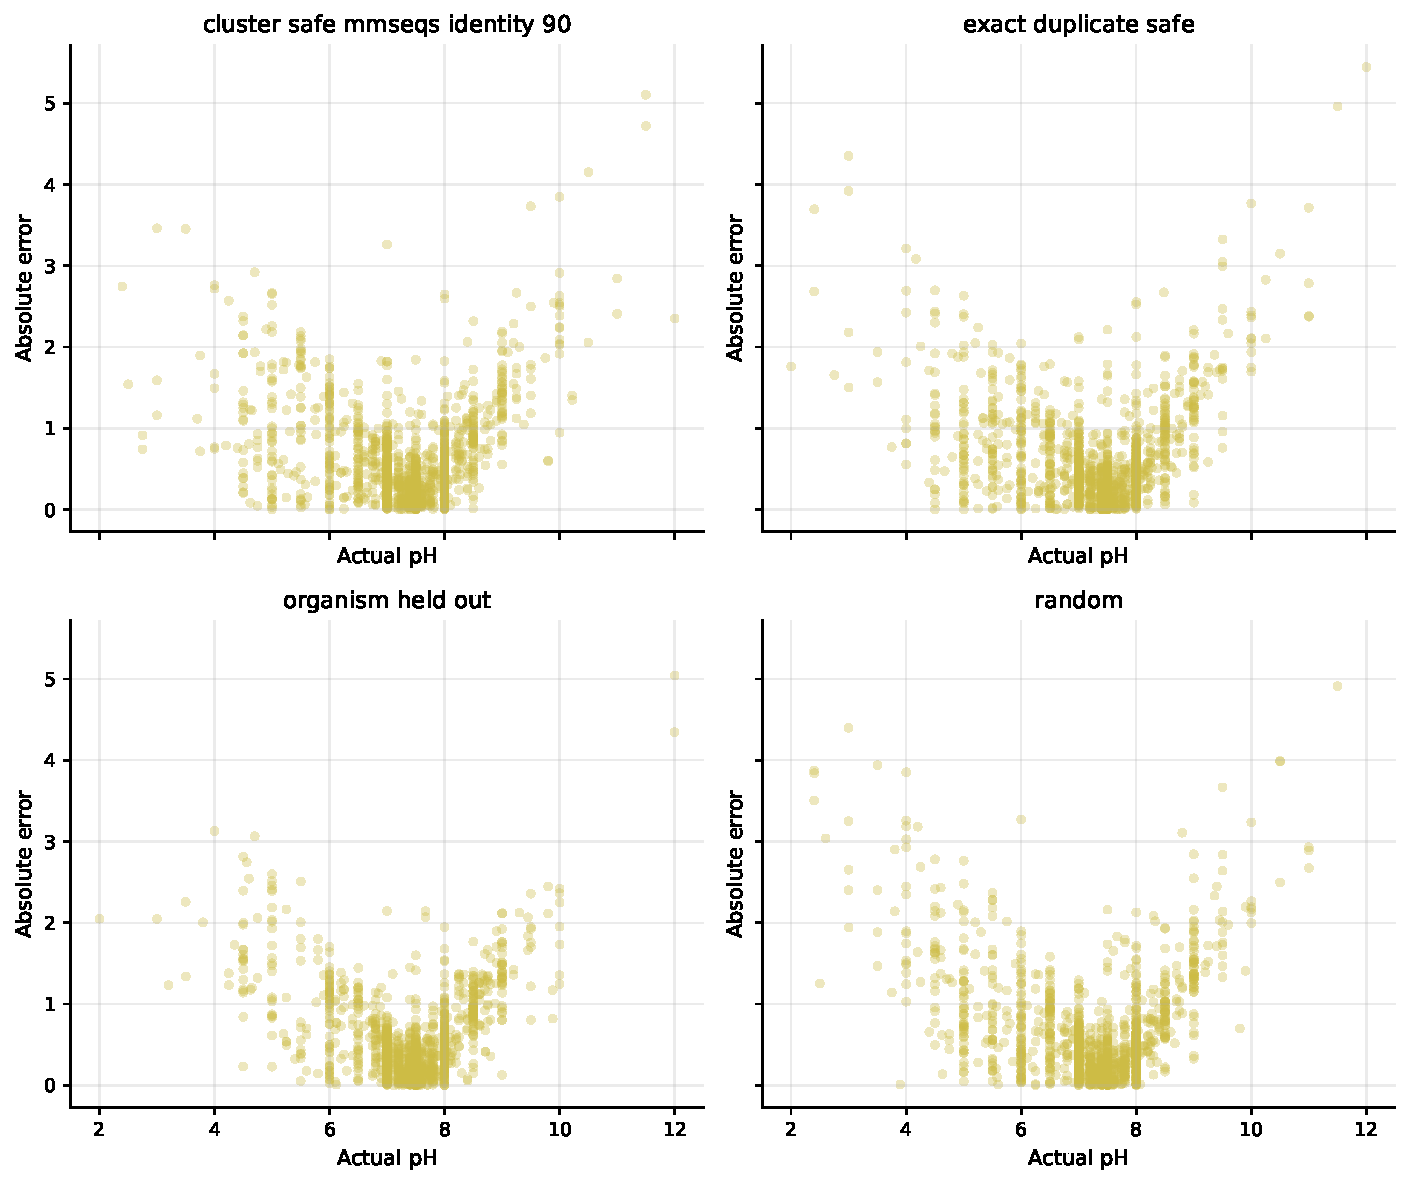
\includegraphics[width=\textwidth]{figures/error_vs_true_ph_best_embedding_models.pdf}
    \caption{Absolute prediction error as a function of true optimal pH for the selected best ESM-2 embedding models. The figure shows the generated diagnostic subset; complete split-strategy results, including the 50\%, 70\%, and EC-held-out evaluations, are reported in the tables.}
    \label{fig:error-vs-true-ph}
\end{figure}

\begin{figure}[htbp]
    \centering
    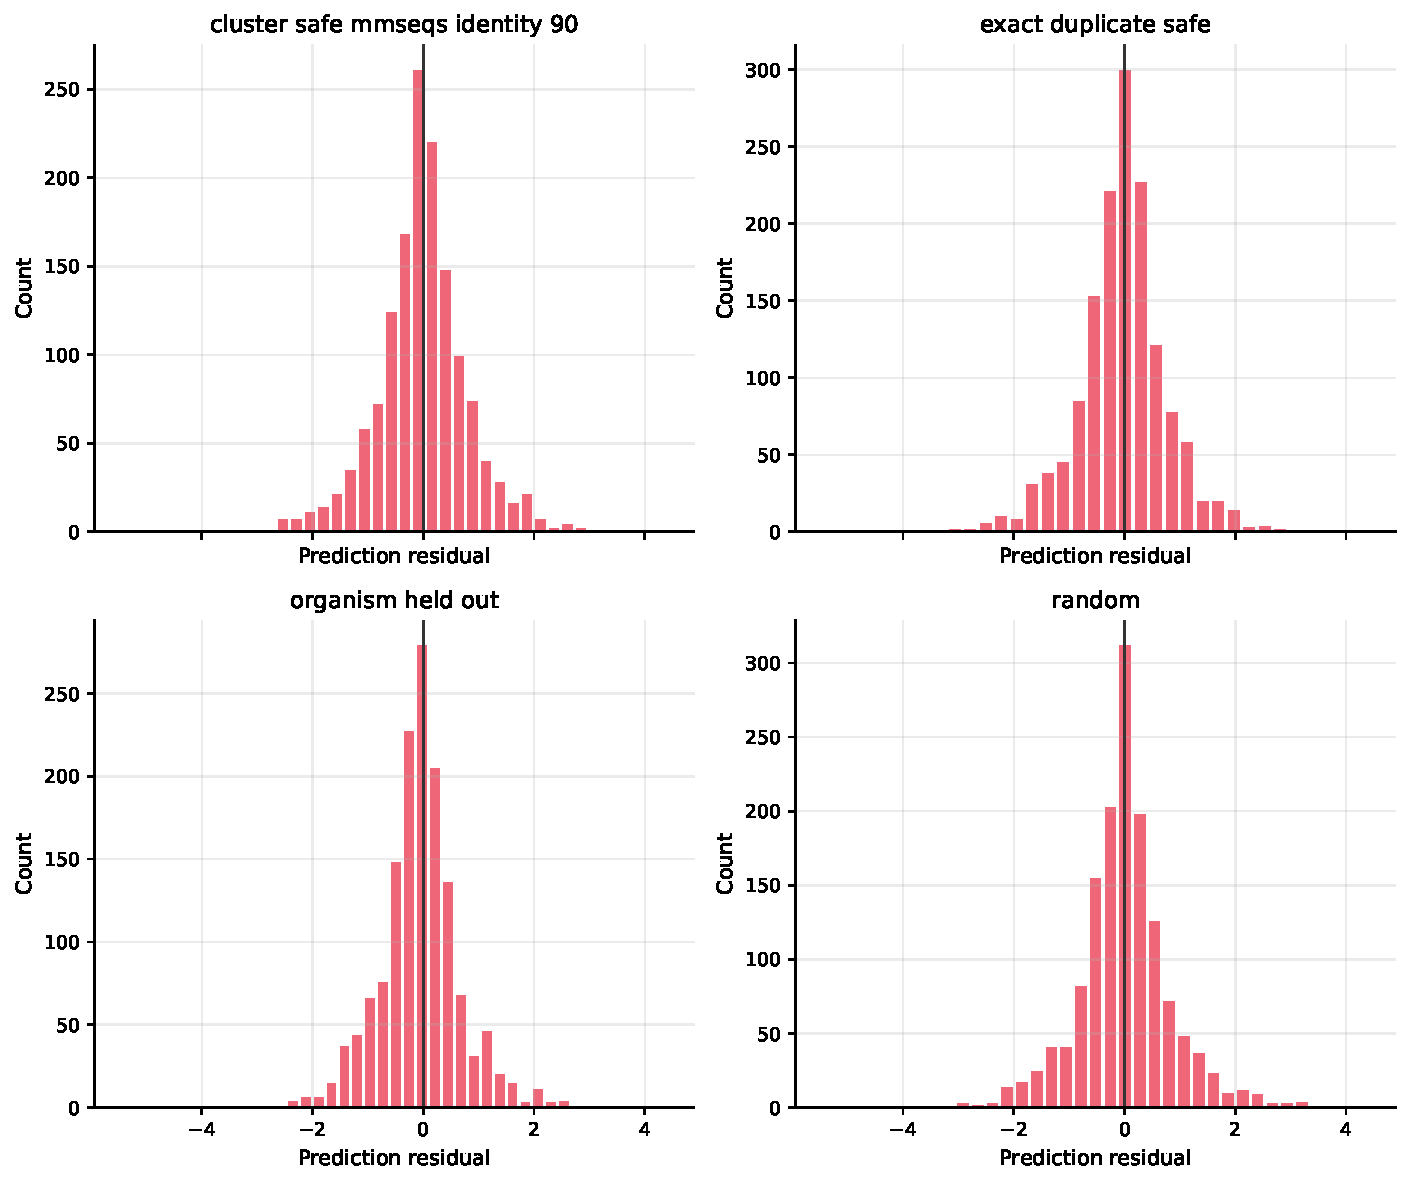
\includegraphics[width=\textwidth]{figures/residual_distribution_best_embedding_models.pdf}
    \caption{Residual distributions for the selected best ESM-2 embedding models. The figure shows the generated diagnostic subset; complete split-strategy results, including the 50\%, 70\%, and EC-held-out evaluations, are reported in the tables.}
    \label{fig:residual-distributions}
\end{figure}

Performance stratified by pH range is reported in Table~\ref{tab:performance-by-ph-range}; acidic, near-neutral, and alkaline are defined as pH $<6$, $6\leq\mathrm{pH}\leq8$, and pH $>8$, respectively. Additional error-analysis tables were exported to the supplementary output directory rather than placed in the main text.

\begin{figure}[htbp]
    \centering
    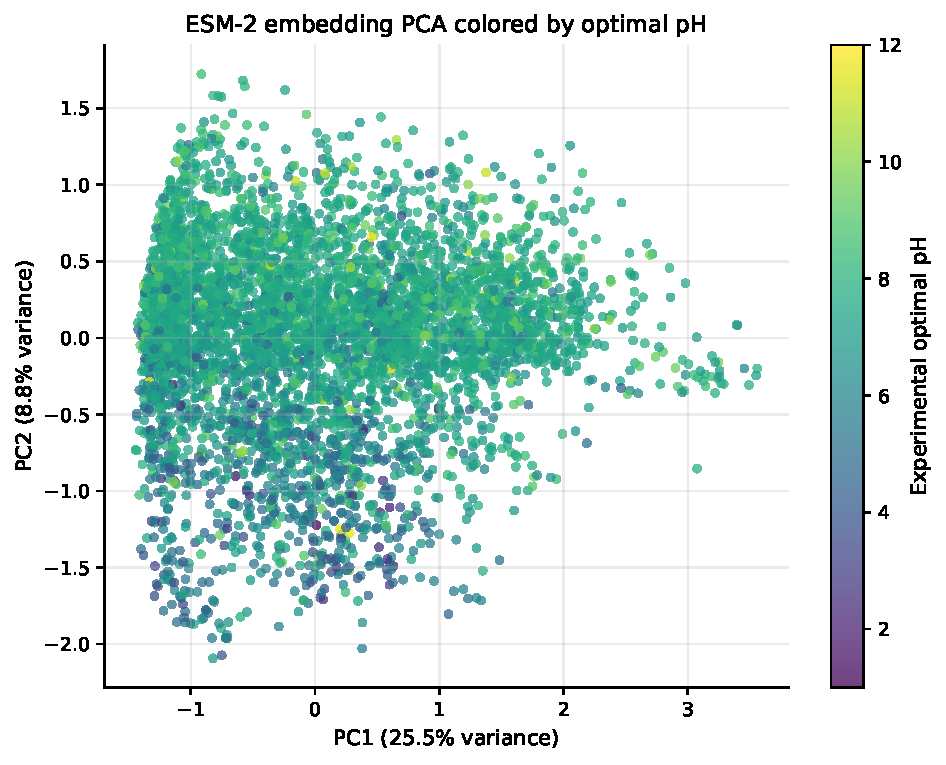
\includegraphics[width=0.78\textwidth]{figures/embedding_pca_optimal_ph.pdf}
    \caption{Principal-component projection of frozen ESM-2 embeddings colored by experimental optimal pH. This visualization is exploratory and does not imply that individual embedding dimensions correspond to biological mechanisms.}
    \label{fig:embedding-pca}
\end{figure}

\begin{figure}[htbp]
    \centering
    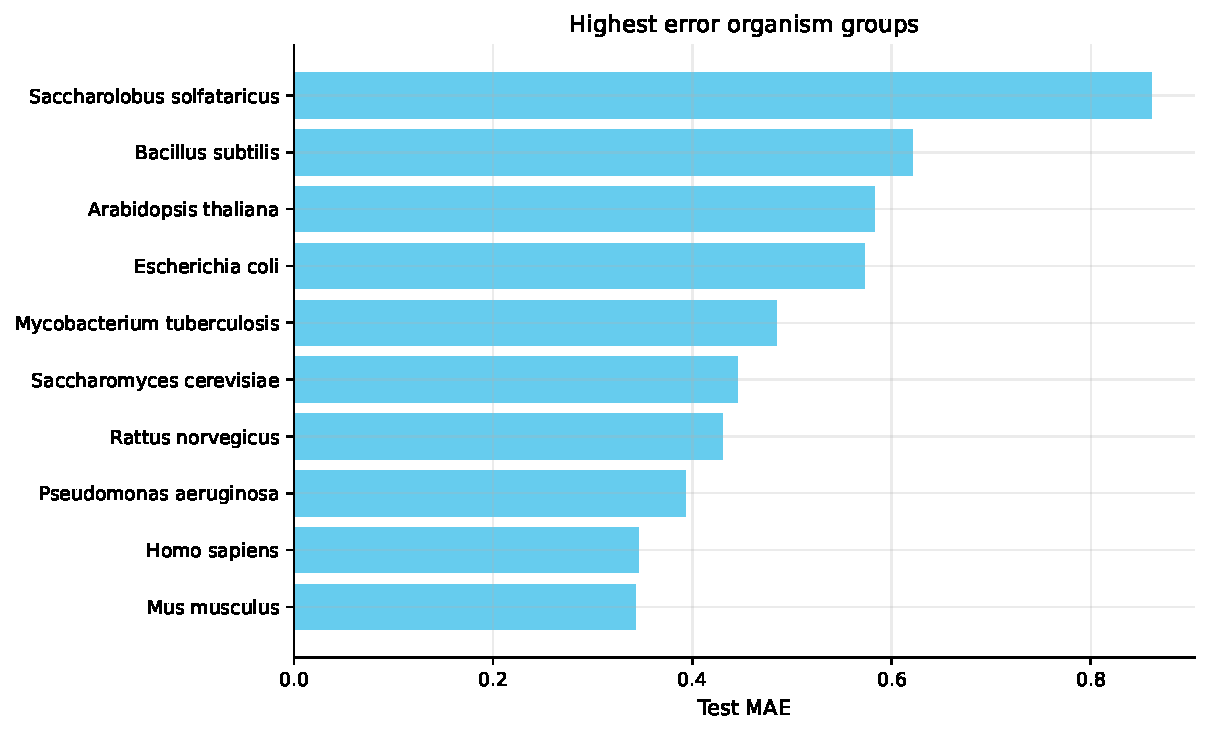
\includegraphics[width=\textwidth]{figures/error_by_organism.pdf}
    \caption{Highest-error organism groups among sufficiently represented test examples for the selected embedding-based model.}
    \label{fig:error-by-organism}
\end{figure}


\section{Discussion}
\label{sec:discussion}
The strongest current empirical result is that frozen ESM-2 embeddings improved predictive accuracy relative to handcrafted sequence features across all non-mean regressors and all evaluated split strategies. This supports the hypothesis that pretrained protein representations can be useful for enzyme optimal-pH prediction. The evidence is strongest for predictive performance, not for mechanistic interpretation.

The split-strategy results are more nuanced. The row-wise random split did contain exact duplicate leakage, yet the 90\% MMseqs2 cluster-safe split did not show worse MAE than the generated random split. Similarly, the organism-held-out split produced lower MAE than the random split. These findings do not support a simple statement that the controlled splits are always harder under the current protocol. The lower-identity MMseqs2 splits were also completed: ESM-2 histogram gradient boosting MAE increased from 0.6148 at 90\% identity to 0.6282 at 70\% and 0.6822 at 50\%. Interpretation remains limited because the organism-held-out test set has lower target-pH variance than the random test set, and cluster composition changes across identity thresholds.

The error analysis suggests that extreme pH labels are associated with large errors, but this pattern must be interpreted in light of label provenance. Zhou and Fang reported disputed pH values and protein-identity assignments in the same EpHod resource \cite{zhou2026caution}; for B5LXD7, the underlying Bispora study reports acidic activity measurements \cite{luo2009novel}, whereas the local file labels the record pH 11.5. This accession is among the largest errors in the 50\% cluster-safe and EC-held-out tests. We therefore do not automatically treat its disagreement as model failure. A leave-one-flagged-record-out sensitivity analysis is reported in \texttt{outputs/metrics/source\_label\_sensitivity.csv}; for the best ESM-2 models, excluding B5LXD7 changes MAE by only -0.0038 on the 50\% split and -0.0037 on the EC-held-out split. This analysis does not correct the label or independently remeasure the original experiment. More generally, extreme-pH error patterns remain compatible with regression toward the mean, but they are not evidence for a causal biochemical mechanism.

The lower-identity cluster experiments provide a more informative stress test. ESM-2 histogram gradient boosting achieved MAE 0.6282 on the 70\% cluster-safe split and 0.6822 on the 50\% split, compared with 0.6148 on the 90\% split. This degradation at lower sequence identity is consistent with a harder sequence-generalization problem, although it does not isolate sequence identity from differences in cluster composition and target distribution.

The EC-held-out experiment provides a complementary test of enzyme-class generalization. Its best ESM-2 model, random forest regression, achieved MAE 0.8321, compared with 0.6250 on the generated random split. This larger error indicates that holding out enzyme classes is considerably more difficult than the current sequence-cluster splits. The comparison should still be interpreted with care because EC groups vary in size and the EC-held-out target distribution may differ from the random test distribution.


\section{Limitations}
\label{sec:limitations}
Several limitations remain. First, the dataset is a curated enzyme optimal-pH resource whose measurements and source annotations were inherited from the EpHod release. Zhou and Fang identified disputed pH values and protein-identity assignments in this resource \cite{zhou2026caution}; our audit confirmed that B5LXD7 is present and quantified its influence, but did not independently recheck every flagged record against every original experiment or alter labels. Consequently, extreme-pH errors should not be interpreted as model failures without source-level verification. Second, taxonomy metadata beyond organism labels were not available in the processed file, so taxonomy-held-out evaluation was limited to organism-held-out splitting. Third, the 50\%, 70\%, and 90\% MMseqs2 cluster thresholds were evaluated, but cluster composition and target-distribution differences still complicate direct comparisons across thresholds.

Fourth, the organism-held-out and EC-held-out splits are group-disjoint but not necessarily distribution-matched. Their test sets may differ in target-pH variance and group-size composition from the generated random test set, which complicates direct MAE comparisons. Fifth, subgroup analyses are limited by sample size; results for rare organisms or EC numbers should not be overinterpreted.

Finally, the ESM-2 embeddings were used as frozen representations with classical regressors. The study does not fine-tune protein-language models, does not reproduce any external model's complete training protocol, and does not claim biological mechanisms from embedding-space or error-analysis patterns.


\section{Conclusion}
\label{sec:conclusion}
This study built a reproducible enzyme optimal-pH prediction pipeline and compared handcrafted sequence features with frozen ESM-2 embeddings under multiple evaluation splits. ESM-2 embeddings improved test MAE across all non-mean regressors and split strategies. The 90\% MMseqs2 cluster-disjoint split and organism-held-out split did not yield higher MAE than the generated random split, so the leakage hypothesis remains unresolved rather than confirmed; nearest-training similarity has not yet been independently audited.

The lower-identity sequence-cluster experiments are complete and show lower ESM-2 performance at 50\% identity than at 70\% and 90\%, consistent with a harder distant-generalization setting. EC-held-out evaluation was substantially harder still: the best ESM-2 model achieved MAE 0.8321 when EC groups were held out. These comparisons remain subject to baseline shifts, row-level dependence, and the source-label concerns documented in the supplementary audit.


\bibliographystyle{plainnat}
\bibliography{references}

\appendix
\section{Supplementary Material}
\label{sec:supplementary}
\subsection{Reproducibility Details}
\label{sec:supplementary-reproducibility}

The CPU-side evaluation was run with Python 3.14.6 on Windows 11. The principal package versions were NumPy 2.5.1, pandas 3.0.5, scikit-learn 1.9.0, SciPy 1.18.0, Biopython 1.87, PyYAML 6.0.3, Matplotlib 3.11.1, seaborn 0.13.2, Jinja2 3.1.6, and pytest 9.1.1. Frozen ESM-2 embeddings were generated in a separate CUDA environment with Python 3.12.13, PyTorch 2.11.0+cu128, model \texttt{facebook/esm2\_t6\_8M\_UR50D}, CUDA, batch size 16, maximum sequence length 1022, 320-dimensional float32 outputs, and 9855 sequences.

The analysis used \texttt{config/default.yaml}. The raw input file \texttt{data/raw/pHopt\_data.csv} was obtained from Zenodo record \texttt{10.5281/zenodo.14252615}, version 1, under CC BY 4.0, and accessed on 2026-10-22 \citep{gado2023phopt}. Its published MD5 is \texttt{d5d0887710e70f2aa5153c15178a6d08}; its local SHA-256 checksum is \texttt{6C2CE7F68E28E4130904A96FC071DBF7FE78E090BD1E408408038F01FA75A3E9}; the cleaned dataset has checksum \texttt{7413D3F48E8A097C4687BA0621F9E4E1D237682FCCAA54B41B952C16E606B3A7}.

Source-label auditing followed the data-quality concerns raised by Zhou and Fang \cite{zhou2026caution}. The named accession B5LXD7 occurs once in the raw file with pHopt 11.5, organism \textit{Bispora sp.}, and EC 3.2.1.78; it occurs in the saved high-error predictions and is a test record for the 50\% cluster-safe and EC-held-out splits. The audit did not overwrite the published label. Instead, a leave-one-flagged-record-out sensitivity analysis was generated by \texttt{scripts/audit\_source\_labels.py}; the accession audit is in \texttt{reports/source\_label\_audit.csv} and the sensitivity results are in \texttt{outputs/metrics/source\_label\_sensitivity.csv}. The original Bispora study is cited as Luo et al. \cite{luo2009novel}.

\subsection{Additional Tables and Figures}
\label{sec:supplementary-additional-results}

Generated supplementary outputs include the complete model-comparison table, the pH-range performance table, bootstrap confidence intervals, paired feature-group comparisons with Holm--Bonferroni-adjusted Wilcoxon p-values, subgroup summaries, and focused error tables under \texttt{outputs/}.

The exhaustive model-comparison table is reproduced below; the main text uses a compact table with readable labels and uncertainty intervals.
\begin{longtable}{lllrrrrrr}
\caption{Test-set performance by feature group, split strategy, and model.} \label{tab:model-comparison} \\
\toprule
feature\_group & split\_strategy & model & n\_examples & mae & rmse & r2 & spearman & pearson \\
\midrule
\endfirsthead
\caption[]{Test-set performance by feature group, split strategy, and model.} \\
\toprule
feature\_group & split\_strategy & model & n\_examples & mae & rmse & r2 & spearman & pearson \\
\midrule
\endhead
\midrule
\multicolumn{9}{r}{Continued on next page} \\
\midrule
\endfoot
\bottomrule
\endlastfoot
esm2\_embedding & cluster\_safe\_mmseqs\_identity\_50 & hist\_gradient\_boosting & 1544 & 0.682200 & 0.998100 & 0.310900 & 0.479300 & 0.561700 \\
esm2\_embedding & cluster\_safe\_mmseqs\_identity\_50 & random\_forest & 1544 & 0.685700 & 1.006900 & 0.298700 & 0.475000 & 0.554100 \\
esm2\_embedding & cluster\_safe\_mmseqs\_identity\_50 & ridge\_regression & 1544 & 0.725100 & 1.022400 & 0.277000 & 0.434100 & 0.529900 \\
handcrafted & cluster\_safe\_mmseqs\_identity\_50 & random\_forest & 1544 & 0.737600 & 1.063900 & 0.217000 & 0.381900 & 0.472000 \\
handcrafted & cluster\_safe\_mmseqs\_identity\_50 & hist\_gradient\_boosting & 1544 & 0.741100 & 1.067100 & 0.212300 & 0.395500 & 0.467200 \\
handcrafted & cluster\_safe\_mmseqs\_identity\_50 & ridge\_regression & 1544 & 0.773900 & 1.106900 & 0.152400 & 0.371000 & 0.398300 \\
esm2\_embedding & cluster\_safe\_mmseqs\_identity\_50 & median\_predictor & 1544 & 0.823800 & 1.253700 & -0.087300 & NaN & NaN \\
handcrafted & cluster\_safe\_mmseqs\_identity\_50 & median\_predictor & 1544 & 0.823800 & 1.253700 & -0.087300 & NaN & NaN \\
esm2\_embedding & cluster\_safe\_mmseqs\_identity\_50 & mean\_predictor & 1544 & 0.851000 & 1.208600 & -0.010400 & NaN & NaN \\
handcrafted & cluster\_safe\_mmseqs\_identity\_50 & mean\_predictor & 1544 & 0.851000 & 1.208600 & -0.010400 & NaN & NaN \\
esm2\_embedding & cluster\_safe\_mmseqs\_identity\_70 & hist\_gradient\_boosting & 1481 & 0.628200 & 0.883700 & 0.407000 & 0.461300 & 0.638700 \\
esm2\_embedding & cluster\_safe\_mmseqs\_identity\_70 & random\_forest & 1481 & 0.629800 & 0.893700 & 0.393500 & 0.473800 & 0.631800 \\
esm2\_embedding & cluster\_safe\_mmseqs\_identity\_70 & ridge\_regression & 1481 & 0.682700 & 0.923100 & 0.353000 & 0.422800 & 0.596400 \\
handcrafted & cluster\_safe\_mmseqs\_identity\_70 & random\_forest & 1481 & 0.695400 & 0.984800 & 0.263600 & 0.375900 & 0.515400 \\
handcrafted & cluster\_safe\_mmseqs\_identity\_70 & hist\_gradient\_boosting & 1481 & 0.701400 & 0.979100 & 0.272100 & 0.376600 & 0.522300 \\
handcrafted & cluster\_safe\_mmseqs\_identity\_70 & ridge\_regression & 1481 & 0.749900 & 1.042800 & 0.174300 & 0.352000 & 0.420800 \\
esm2\_embedding & cluster\_safe\_mmseqs\_identity\_70 & median\_predictor & 1481 & 0.781800 & 1.172600 & -0.044100 & NaN & NaN \\
handcrafted & cluster\_safe\_mmseqs\_identity\_70 & median\_predictor & 1481 & 0.781800 & 1.172600 & -0.044100 & NaN & NaN \\
esm2\_embedding & cluster\_safe\_mmseqs\_identity\_70 & mean\_predictor & 1481 & 0.812800 & 1.148000 & -0.000600 & NaN & NaN \\
handcrafted & cluster\_safe\_mmseqs\_identity\_70 & mean\_predictor & 1481 & 0.812800 & 1.148000 & -0.000600 & NaN & NaN \\
esm2\_embedding & cluster\_safe\_mmseqs\_identity\_90 & hist\_gradient\_boosting & 1473 & 0.614800 & 0.868300 & 0.414400 & 0.513300 & 0.644500 \\
esm2\_embedding & cluster\_safe\_mmseqs\_identity\_90 & random\_forest & 1473 & 0.616400 & 0.881900 & 0.395900 & 0.515400 & 0.633000 \\
esm2\_embedding & cluster\_safe\_mmseqs\_identity\_90 & ridge\_regression & 1473 & 0.678600 & 0.924800 & 0.335700 & 0.450600 & 0.582900 \\
handcrafted & cluster\_safe\_mmseqs\_identity\_90 & random\_forest & 1473 & 0.681300 & 0.959700 & 0.284600 & 0.402900 & 0.535300 \\
handcrafted & cluster\_safe\_mmseqs\_identity\_90 & hist\_gradient\_boosting & 1473 & 0.705200 & 0.976600 & 0.259200 & 0.359100 & 0.511700 \\
handcrafted & cluster\_safe\_mmseqs\_identity\_90 & ridge\_regression & 1473 & 0.756000 & 1.035100 & 0.167900 & 0.321700 & 0.411200 \\
esm2\_embedding & cluster\_safe\_mmseqs\_identity\_90 & median\_predictor & 1473 & 0.781900 & 1.155600 & -0.037300 & NaN & NaN \\
handcrafted & cluster\_safe\_mmseqs\_identity\_90 & median\_predictor & 1473 & 0.781900 & 1.155600 & -0.037300 & NaN & NaN \\
esm2\_embedding & cluster\_safe\_mmseqs\_identity\_90 & mean\_predictor & 1473 & 0.817800 & 1.136400 & -0.003000 & NaN & NaN \\
handcrafted & cluster\_safe\_mmseqs\_identity\_90 & mean\_predictor & 1473 & 0.817800 & 1.136400 & -0.003000 & NaN & NaN \\
esm2\_embedding & dataset\_provided & random\_forest & 1971 & 0.603500 & 0.849100 & 0.459200 & 0.598800 & 0.691300 \\
esm2\_embedding & dataset\_provided & hist\_gradient\_boosting & 1971 & 0.613200 & 0.857200 & 0.448800 & 0.574800 & 0.672300 \\
handcrafted & dataset\_provided & random\_forest & 1971 & 0.672700 & 0.934300 & 0.345100 & 0.483100 & 0.595100 \\
esm2\_embedding & dataset\_provided & ridge\_regression & 1971 & 0.674200 & 0.912500 & 0.375300 & 0.497300 & 0.613800 \\
handcrafted & dataset\_provided & hist\_gradient\_boosting & 1971 & 0.688300 & 0.944500 & 0.330700 & 0.451100 & 0.578100 \\
handcrafted & dataset\_provided & ridge\_regression & 1971 & 0.757300 & 1.020300 & 0.219100 & 0.380900 & 0.472800 \\
esm2\_embedding & dataset\_provided & median\_predictor & 1971 & 0.809700 & 1.181700 & -0.047600 & NaN & NaN \\
handcrafted & dataset\_provided & median\_predictor & 1971 & 0.809700 & 1.181700 & -0.047600 & NaN & NaN \\
esm2\_embedding & dataset\_provided & mean\_predictor & 1971 & 0.848100 & 1.155200 & -0.001100 & NaN & NaN \\
handcrafted & dataset\_provided & mean\_predictor & 1971 & 0.848100 & 1.155200 & -0.001100 & NaN & NaN \\
esm2\_embedding & ec\_held\_out & random\_forest & 1478 & 0.832100 & 1.188800 & 0.233300 & 0.511200 & 0.496400 \\
esm2\_embedding & ec\_held\_out & ridge\_regression & 1478 & 0.839500 & 1.161400 & 0.268200 & 0.527500 & 0.525100 \\
esm2\_embedding & ec\_held\_out & hist\_gradient\_boosting & 1478 & 0.840900 & 1.195200 & 0.225100 & 0.501700 & 0.494400 \\
handcrafted & ec\_held\_out & random\_forest & 1478 & 0.884400 & 1.211800 & 0.203400 & 0.479200 & 0.483300 \\
handcrafted & ec\_held\_out & hist\_gradient\_boosting & 1478 & 0.913900 & 1.241200 & 0.164300 & 0.437600 & 0.456100 \\
handcrafted & ec\_held\_out & ridge\_regression & 1478 & 0.933900 & 1.257000 & 0.142900 & 0.470400 & 0.454800 \\
esm2\_embedding & ec\_held\_out & mean\_predictor & 1478 & 1.099700 & 1.486500 & -0.198800 & NaN & NaN \\
handcrafted & ec\_held\_out & mean\_predictor & 1478 & 1.099700 & 1.486500 & -0.198800 & NaN & NaN \\
esm2\_embedding & ec\_held\_out & median\_predictor & 1478 & 1.134300 & 1.551900 & -0.306600 & NaN & NaN \\
handcrafted & ec\_held\_out & median\_predictor & 1478 & 1.134300 & 1.551900 & -0.306600 & NaN & NaN \\
esm2\_embedding & exact\_duplicate\_safe & hist\_gradient\_boosting & 1480 & 0.602800 & 0.862500 & 0.440300 & 0.560000 & 0.665000 \\
esm2\_embedding & exact\_duplicate\_safe & random\_forest & 1480 & 0.607300 & 0.871700 & 0.428200 & 0.562600 & 0.662200 \\
handcrafted & exact\_duplicate\_safe & random\_forest & 1480 & 0.663800 & 0.944300 & 0.329000 & 0.482000 & 0.578400 \\
handcrafted & exact\_duplicate\_safe & hist\_gradient\_boosting & 1480 & 0.679700 & 0.953700 & 0.315600 & 0.463400 & 0.562900 \\
esm2\_embedding & exact\_duplicate\_safe & ridge\_regression & 1480 & 0.686300 & 0.943600 & 0.330000 & 0.470000 & 0.577600 \\
handcrafted & exact\_duplicate\_safe & ridge\_regression & 1480 & 0.751800 & 1.036900 & 0.190900 & 0.379400 & 0.439900 \\
esm2\_embedding & exact\_duplicate\_safe & median\_predictor & 1480 & 0.798400 & 1.179100 & -0.046100 & NaN & NaN \\
handcrafted & exact\_duplicate\_safe & median\_predictor & 1480 & 0.798400 & 1.179100 & -0.046100 & NaN & NaN \\
esm2\_embedding & exact\_duplicate\_safe & mean\_predictor & 1480 & 0.837100 & 1.153200 & -0.000700 & NaN & NaN \\
handcrafted & exact\_duplicate\_safe & mean\_predictor & 1480 & 0.837100 & 1.153200 & -0.000700 & NaN & NaN \\
esm2\_embedding & organism\_held\_out & random\_forest & 1478 & 0.536000 & 0.758500 & 0.359000 & 0.457700 & 0.605500 \\
esm2\_embedding & organism\_held\_out & hist\_gradient\_boosting & 1478 & 0.538600 & 0.754100 & 0.366400 & 0.455300 & 0.606200 \\
handcrafted & organism\_held\_out & random\_forest & 1478 & 0.594400 & 0.837400 & 0.218700 & 0.367100 & 0.474100 \\
handcrafted & organism\_held\_out & hist\_gradient\_boosting & 1478 & 0.605200 & 0.842600 & 0.208900 & 0.335500 & 0.464500 \\
esm2\_embedding & organism\_held\_out & ridge\_regression & 1478 & 0.620900 & 0.835200 & 0.222700 & 0.386800 & 0.502600 \\
esm2\_embedding & organism\_held\_out & median\_predictor & 1478 & 0.630600 & 0.947400 & -0.000100 & NaN & NaN \\
handcrafted & organism\_held\_out & median\_predictor & 1478 & 0.630600 & 0.947400 & -0.000100 & NaN & NaN \\
handcrafted & organism\_held\_out & ridge\_regression & 1478 & 0.659300 & 0.907600 & 0.082200 & 0.286200 & 0.345800 \\
esm2\_embedding & organism\_held\_out & mean\_predictor & 1478 & 0.709900 & 0.973900 & -0.056900 & NaN & NaN \\
handcrafted & organism\_held\_out & mean\_predictor & 1478 & 0.709900 & 0.973900 & -0.056900 & NaN & NaN \\
esm2\_embedding & random & random\_forest & 1479 & 0.625000 & 0.911400 & 0.407600 & 0.539300 & 0.645900 \\
esm2\_embedding & random & hist\_gradient\_boosting & 1479 & 0.633500 & 0.907900 & 0.412100 & 0.514900 & 0.643300 \\
handcrafted & random & random\_forest & 1479 & 0.698400 & 1.011400 & 0.270500 & 0.432900 & 0.520300 \\
esm2\_embedding & random & ridge\_regression & 1479 & 0.703500 & 0.975000 & 0.322000 & 0.453300 & 0.567900 \\
handcrafted & random & hist\_gradient\_boosting & 1479 & 0.709100 & 1.004900 & 0.279800 & 0.414600 & 0.530300 \\
handcrafted & random & ridge\_regression & 1479 & 0.781700 & 1.082900 & 0.163700 & 0.333200 & 0.405000 \\
esm2\_embedding & random & median\_predictor & 1479 & 0.812700 & 1.218400 & -0.058700 & NaN & NaN \\
handcrafted & random & median\_predictor & 1479 & 0.812700 & 1.218400 & -0.058700 & NaN & NaN \\
esm2\_embedding & random & mean\_predictor & 1479 & 0.844400 & 1.184300 & -0.000200 & NaN & NaN \\
handcrafted & random & mean\_predictor & 1479 & 0.844400 & 1.184300 & -0.000200 & NaN & NaN \\
\end{longtable}



\end{document}
